% Options for packages loaded elsewhere
% Options for packages loaded elsewhere
\PassOptionsToPackage{unicode}{hyperref}
\PassOptionsToPackage{hyphens}{url}
\PassOptionsToPackage{dvipsnames,svgnames,x11names}{xcolor}
%
\documentclass[
  letterpaper,
  DIV=11,
  numbers=noendperiod]{scrartcl}
\usepackage{xcolor}
\usepackage[margin=1in]{geometry}
\usepackage{amsmath,amssymb}
\setcounter{secnumdepth}{5}
\usepackage{iftex}
\ifPDFTeX
  \usepackage[T1]{fontenc}
  \usepackage[utf8]{inputenc}
  \usepackage{textcomp} % provide euro and other symbols
\else % if luatex or xetex
  \usepackage{unicode-math} % this also loads fontspec
  \defaultfontfeatures{Scale=MatchLowercase}
  \defaultfontfeatures[\rmfamily]{Ligatures=TeX,Scale=1}
\fi
\usepackage{lmodern}
\ifPDFTeX\else
  % xetex/luatex font selection
  \setmainfont[]{Garamond}
\fi
% Use upquote if available, for straight quotes in verbatim environments
\IfFileExists{upquote.sty}{\usepackage{upquote}}{}
\IfFileExists{microtype.sty}{% use microtype if available
  \usepackage[]{microtype}
  \UseMicrotypeSet[protrusion]{basicmath} % disable protrusion for tt fonts
}{}
\makeatletter
\@ifundefined{KOMAClassName}{% if non-KOMA class
  \IfFileExists{parskip.sty}{%
    \usepackage{parskip}
  }{% else
    \setlength{\parindent}{0pt}
    \setlength{\parskip}{6pt plus 2pt minus 1pt}}
}{% if KOMA class
  \KOMAoptions{parskip=half}}
\makeatother
% Make \paragraph and \subparagraph free-standing
\makeatletter
\ifx\paragraph\undefined\else
  \let\oldparagraph\paragraph
  \renewcommand{\paragraph}{
    \@ifstar
      \xxxParagraphStar
      \xxxParagraphNoStar
  }
  \newcommand{\xxxParagraphStar}[1]{\oldparagraph*{#1}\mbox{}}
  \newcommand{\xxxParagraphNoStar}[1]{\oldparagraph{#1}\mbox{}}
\fi
\ifx\subparagraph\undefined\else
  \let\oldsubparagraph\subparagraph
  \renewcommand{\subparagraph}{
    \@ifstar
      \xxxSubParagraphStar
      \xxxSubParagraphNoStar
  }
  \newcommand{\xxxSubParagraphStar}[1]{\oldsubparagraph*{#1}\mbox{}}
  \newcommand{\xxxSubParagraphNoStar}[1]{\oldsubparagraph{#1}\mbox{}}
\fi
\makeatother


\usepackage{longtable,booktabs,array}
\usepackage{calc} % for calculating minipage widths
% Correct order of tables after \paragraph or \subparagraph
\usepackage{etoolbox}
\makeatletter
\patchcmd\longtable{\par}{\if@noskipsec\mbox{}\fi\par}{}{}
\makeatother
% Allow footnotes in longtable head/foot
\IfFileExists{footnotehyper.sty}{\usepackage{footnotehyper}}{\usepackage{footnote}}
\makesavenoteenv{longtable}
\usepackage{graphicx}
\makeatletter
\newsavebox\pandoc@box
\newcommand*\pandocbounded[1]{% scales image to fit in text height/width
  \sbox\pandoc@box{#1}%
  \Gscale@div\@tempa{\textheight}{\dimexpr\ht\pandoc@box+\dp\pandoc@box\relax}%
  \Gscale@div\@tempb{\linewidth}{\wd\pandoc@box}%
  \ifdim\@tempb\p@<\@tempa\p@\let\@tempa\@tempb\fi% select the smaller of both
  \ifdim\@tempa\p@<\p@\scalebox{\@tempa}{\usebox\pandoc@box}%
  \else\usebox{\pandoc@box}%
  \fi%
}
% Set default figure placement to htbp
\def\fps@figure{htbp}
\makeatother





\setlength{\emergencystretch}{3em} % prevent overfull lines

\providecommand{\tightlist}{%
  \setlength{\itemsep}{0pt}\setlength{\parskip}{0pt}}



 


% header.tex

\usepackage{xcolor}
\usepackage{pagecolor}
\usepackage{float} % to control figure positions
\usepackage{booktabs} % for nicer tables
\usepackage{caption}
\usepackage{fancyhdr}
\usepackage{graphicx}

\pagestyle{fancy}

\fancyhead{} % clear all header fields
\fancyhead[R]{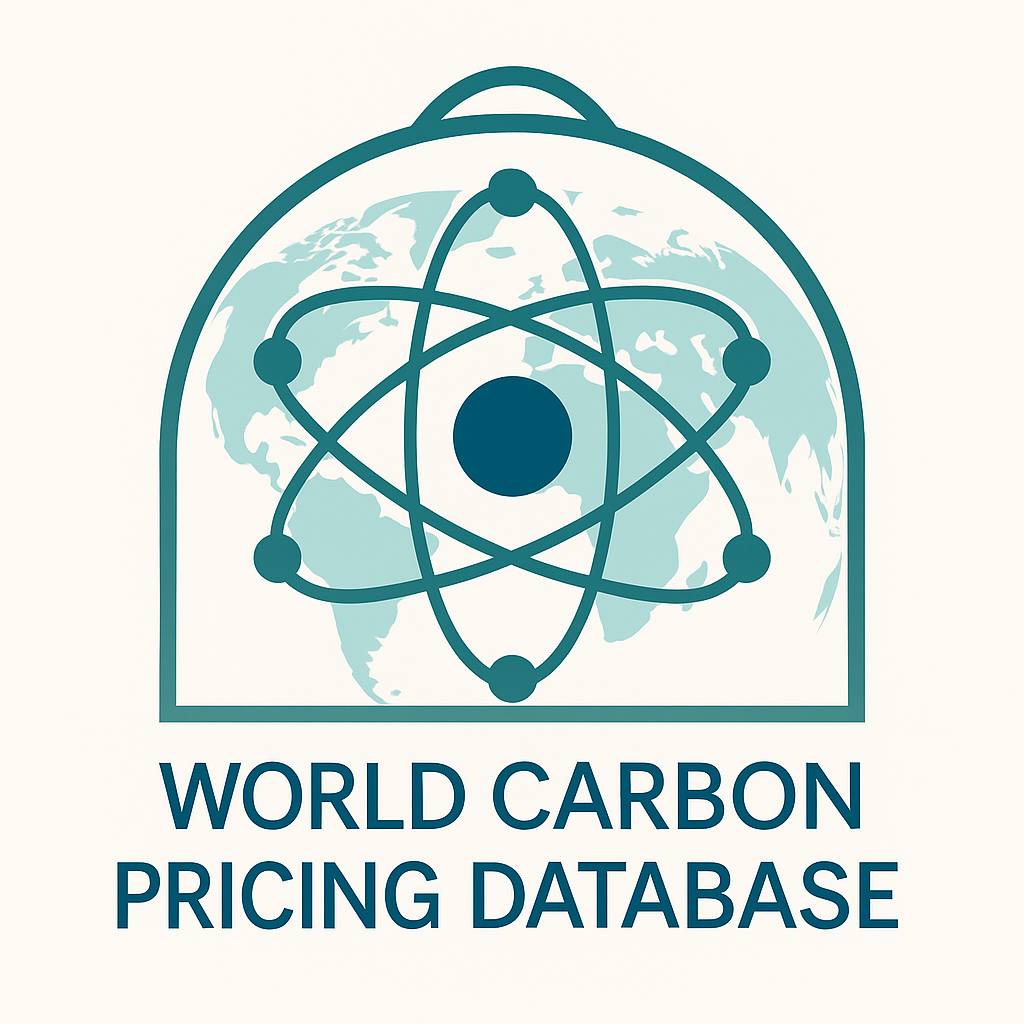
\includegraphics[width=1cm]{/Users/gd/GitHub/ECP/_output/_reports/wcpd_new.png}}

\renewcommand{\headrulewidth}{0pt}

\definecolor{offwhite}{RGB}{253,252,248} % adjust as you like
\pagecolor{offwhite}


\captionsetup{font=small, labelfont=bf}
\KOMAoption{captions}{tableheading}
\makeatletter
\@ifpackageloaded{caption}{}{\usepackage{caption}}
\AtBeginDocument{%
\ifdefined\contentsname
  \renewcommand*\contentsname{Table of contents}
\else
  \newcommand\contentsname{Table of contents}
\fi
\ifdefined\listfigurename
  \renewcommand*\listfigurename{List of Figures}
\else
  \newcommand\listfigurename{List of Figures}
\fi
\ifdefined\listtablename
  \renewcommand*\listtablename{List of Tables}
\else
  \newcommand\listtablename{List of Tables}
\fi
\ifdefined\figurename
  \renewcommand*\figurename{Figure}
\else
  \newcommand\figurename{Figure}
\fi
\ifdefined\tablename
  \renewcommand*\tablename{Table}
\else
  \newcommand\tablename{Table}
\fi
}
\@ifpackageloaded{float}{}{\usepackage{float}}
\floatstyle{ruled}
\@ifundefined{c@chapter}{\newfloat{codelisting}{h}{lop}}{\newfloat{codelisting}{h}{lop}[chapter]}
\floatname{codelisting}{Listing}
\newcommand*\listoflistings{\listof{codelisting}{List of Listings}}
\makeatother
\makeatletter
\makeatother
\makeatletter
\@ifpackageloaded{caption}{}{\usepackage{caption}}
\@ifpackageloaded{subcaption}{}{\usepackage{subcaption}}
\makeatother
\usepackage{bookmark}
\IfFileExists{xurl.sty}{\usepackage{xurl}}{} % add URL line breaks if available
\urlstyle{same}
\hypersetup{
  pdftitle={World Carbon Pricing Database Report},
  colorlinks=true,
  linkcolor={blue},
  filecolor={Maroon},
  citecolor={Blue},
  urlcolor={Blue},
  pdfcreator={LaTeX via pandoc}}


\title{World Carbon Pricing Database Report}
\author{}
\date{}
\begin{document}
\maketitle

\renewcommand*\contentsname{Table of contents}
{
\hypersetup{linkcolor=}
\setcounter{tocdepth}{2}
\tableofcontents
}

\subsection*{Report version}\label{report-version}

\textbf{July} \textbf{2025}.

\subsection*{Contact}\label{contact}

\textbf{Name:} Geoffroy Dolphin\\
\textbf{Email:} gdolphin@rff.org\\
\textbf{Website:} \url{geoffoydolphin.eu}

\subsection*{Disclaimer}\label{disclaimer}

This report is based on the latest update of the World Carbon Pricing
Database and the associated emissions-weighted carbon price. The data
presented in this report is licensed under a
Attribution-NonCommercial-NoDerivatives 4.0 International (CC BY-NC-ND
4.0). For any commercial use, please contact the author.

\newpage

\tableofcontents

\listoffigures

\listoftables

\newpage

\section{Cross-country summary}\label{cross-country-summary}

\begin{longtable}[]{@{}lllllll@{}}

\caption{\label{tbl-summary}Summary statistics for 2020-2024}

\tabularnewline

\caption{}\label{T_a07a4}\tabularnewline
\toprule\noalign{}
group & & 2020 & 2021 & 2022 & 2023 & 2024 \\
\midrule\noalign{}
\endfirsthead
\toprule\noalign{}
group & & 2020 & 2021 & 2022 & 2023 & 2024 \\
\midrule\noalign{}
\endhead
\bottomrule\noalign{}
\endlastfoot
All & count & 297.00 & 297.00 & 297.00 & 297.00 & 297.00 \\
& max & 84.01 & 107.19 & 129.33 & 133.43 & 141.16 \\
& mean & 3.70 & 5.59 & 7.47 & 7.67 & 7.33 \\
& median & 0.00 & 0.00 & 0.00 & 0.00 & 0.00 \\
& min & 0.00 & 0.00 & 0.00 & 0.00 & 0.00 \\
& std & 10.44 & 14.62 & 19.36 & 19.99 & 19.42 \\
AsiaPacific & count & 39.00 & 39.00 & 39.00 & 39.00 & 39.00 \\
& max & 18.49 & 28.18 & 40.11 & 30.31 & 28.96 \\
& mean & 0.62 & 0.91 & 1.25 & 1.01 & 1.27 \\
& median & 0.00 & 0.00 & 0.00 & 0.00 & 0.00 \\
& min & 0.00 & 0.00 & 0.00 & 0.00 & 0.00 \\
& std & 2.99 & 4.53 & 6.43 & 4.88 & 5.03 \\
EU27 & count & 26.00 & 26.00 & 26.00 & 26.00 & 26.00 \\
& max & 83.13 & 107.19 & 119.23 & 120.28 & 118.26 \\
& mean & 22.14 & 39.97 & 52.80 & 52.10 & 44.30 \\
& median & 15.66 & 37.04 & 51.88 & 50.20 & 39.07 \\
& min & 7.76 & 18.53 & 23.30 & 22.82 & 17.79 \\
& std & 18.62 & 20.05 & 21.34 & 21.86 & 23.29 \\
MiddleIncome & count & 105.00 & 105.00 & 105.00 & 105.00 & 105.00 \\
& max & 19.08 & 40.38 & 55.02 & 53.13 & 41.16 \\
& mean & 0.49 & 0.84 & 1.06 & 0.99 & 0.84 \\
& median & 0.00 & 0.00 & 0.00 & 0.00 & 0.00 \\
& min & 0.00 & 0.00 & 0.00 & 0.00 & 0.00 \\
& std & 2.54 & 5.00 & 6.56 & 6.26 & 4.96 \\
OECD & count & 36.00 & 36.00 & 36.00 & 36.00 & 36.00 \\
& max & 84.01 & 107.19 & 119.23 & 126.02 & 137.02 \\
& mean & 20.13 & 32.15 & 40.93 & 40.44 & 36.01 \\
& median & 15.11 & 28.16 & 40.93 & 39.93 & 31.32 \\
& min & 0.00 & 0.00 & 0.00 & 0.00 & 0.00 \\
& std & 21.07 & 25.30 & 29.10 & 31.49 & 31.72 \\

\end{longtable}

\subsection{Coverage}\label{coverage}

\subsubsection{\texorpdfstring{CO\(_2\)}{CO\_2}}\label{co_2}

\begin{figure}

\centering{

\pandocbounded{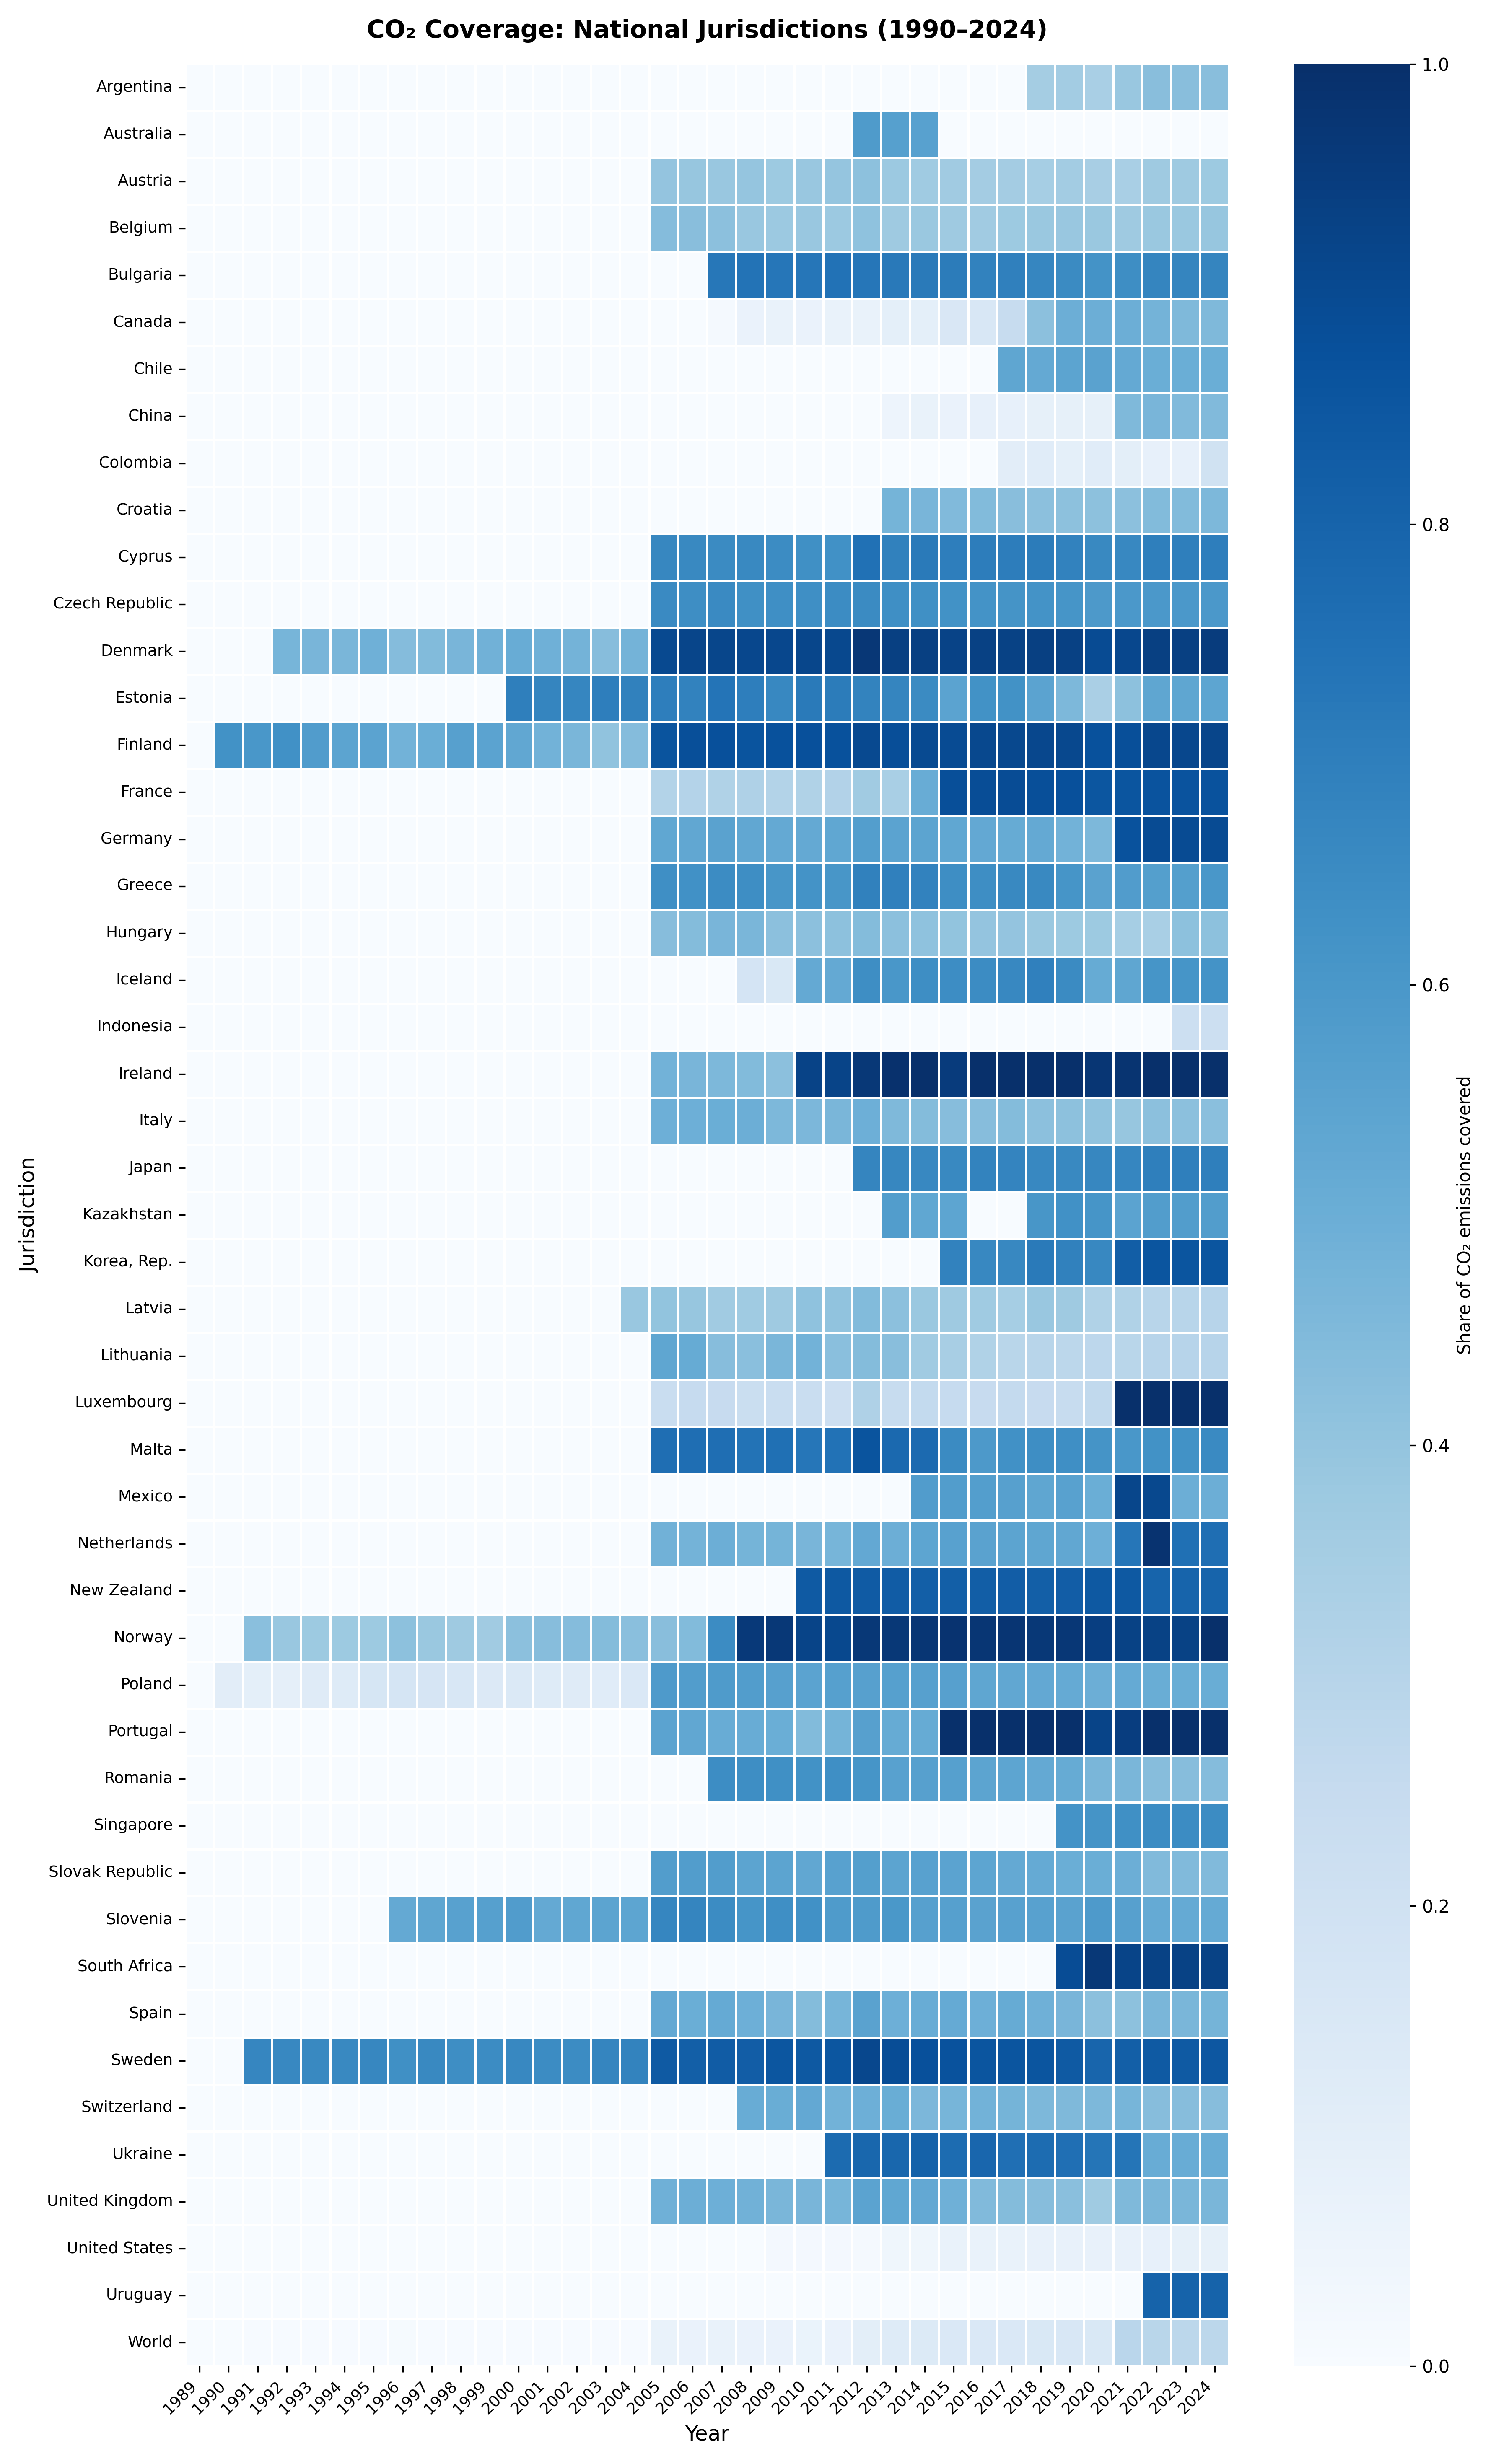
\includegraphics[keepaspectratio]{../../../_output/_figures/plots/coverage_hm_national.png}}

}

\caption{\label{fig-heatmap-coverage-national}Carbon pricing CO\(_2\)
coverage --- Countries, 1990--2024}

\end{figure}%

\begin{figure}

\centering{

\pandocbounded{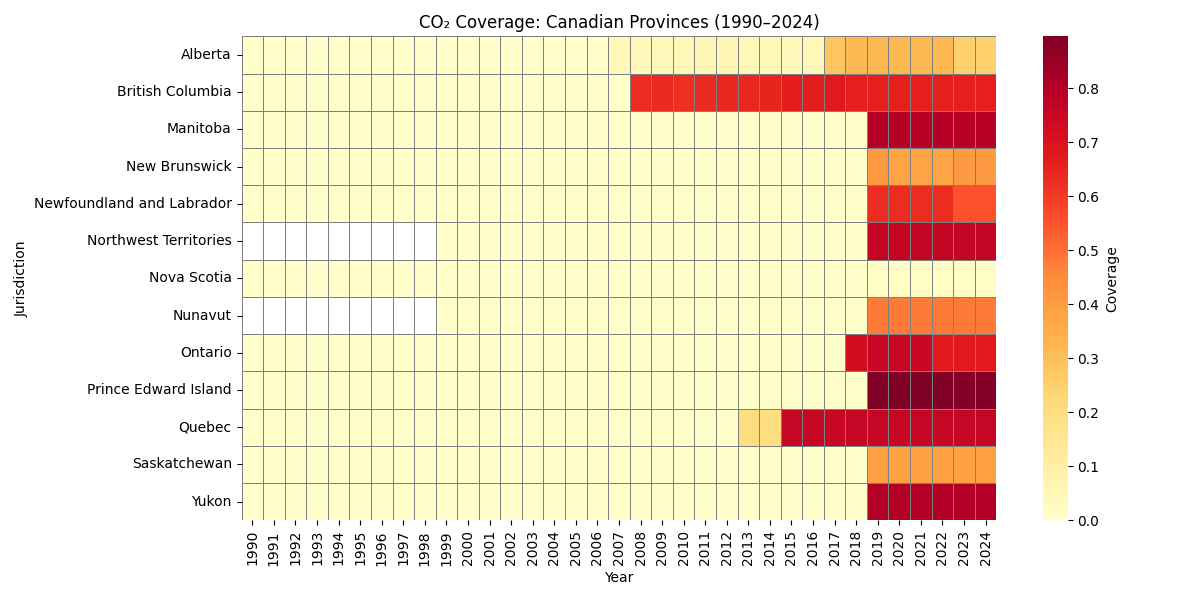
\includegraphics[keepaspectratio]{../../../_output/_figures/plots/coverage_hm_canada.png}}

}

\caption{\label{fig-heatmap-coverage-canada}Carbon pricing CO\(_2\)
coverage --- Canadian provinces, 1990--2024}

\end{figure}%

\begin{figure}

\centering{

\pandocbounded{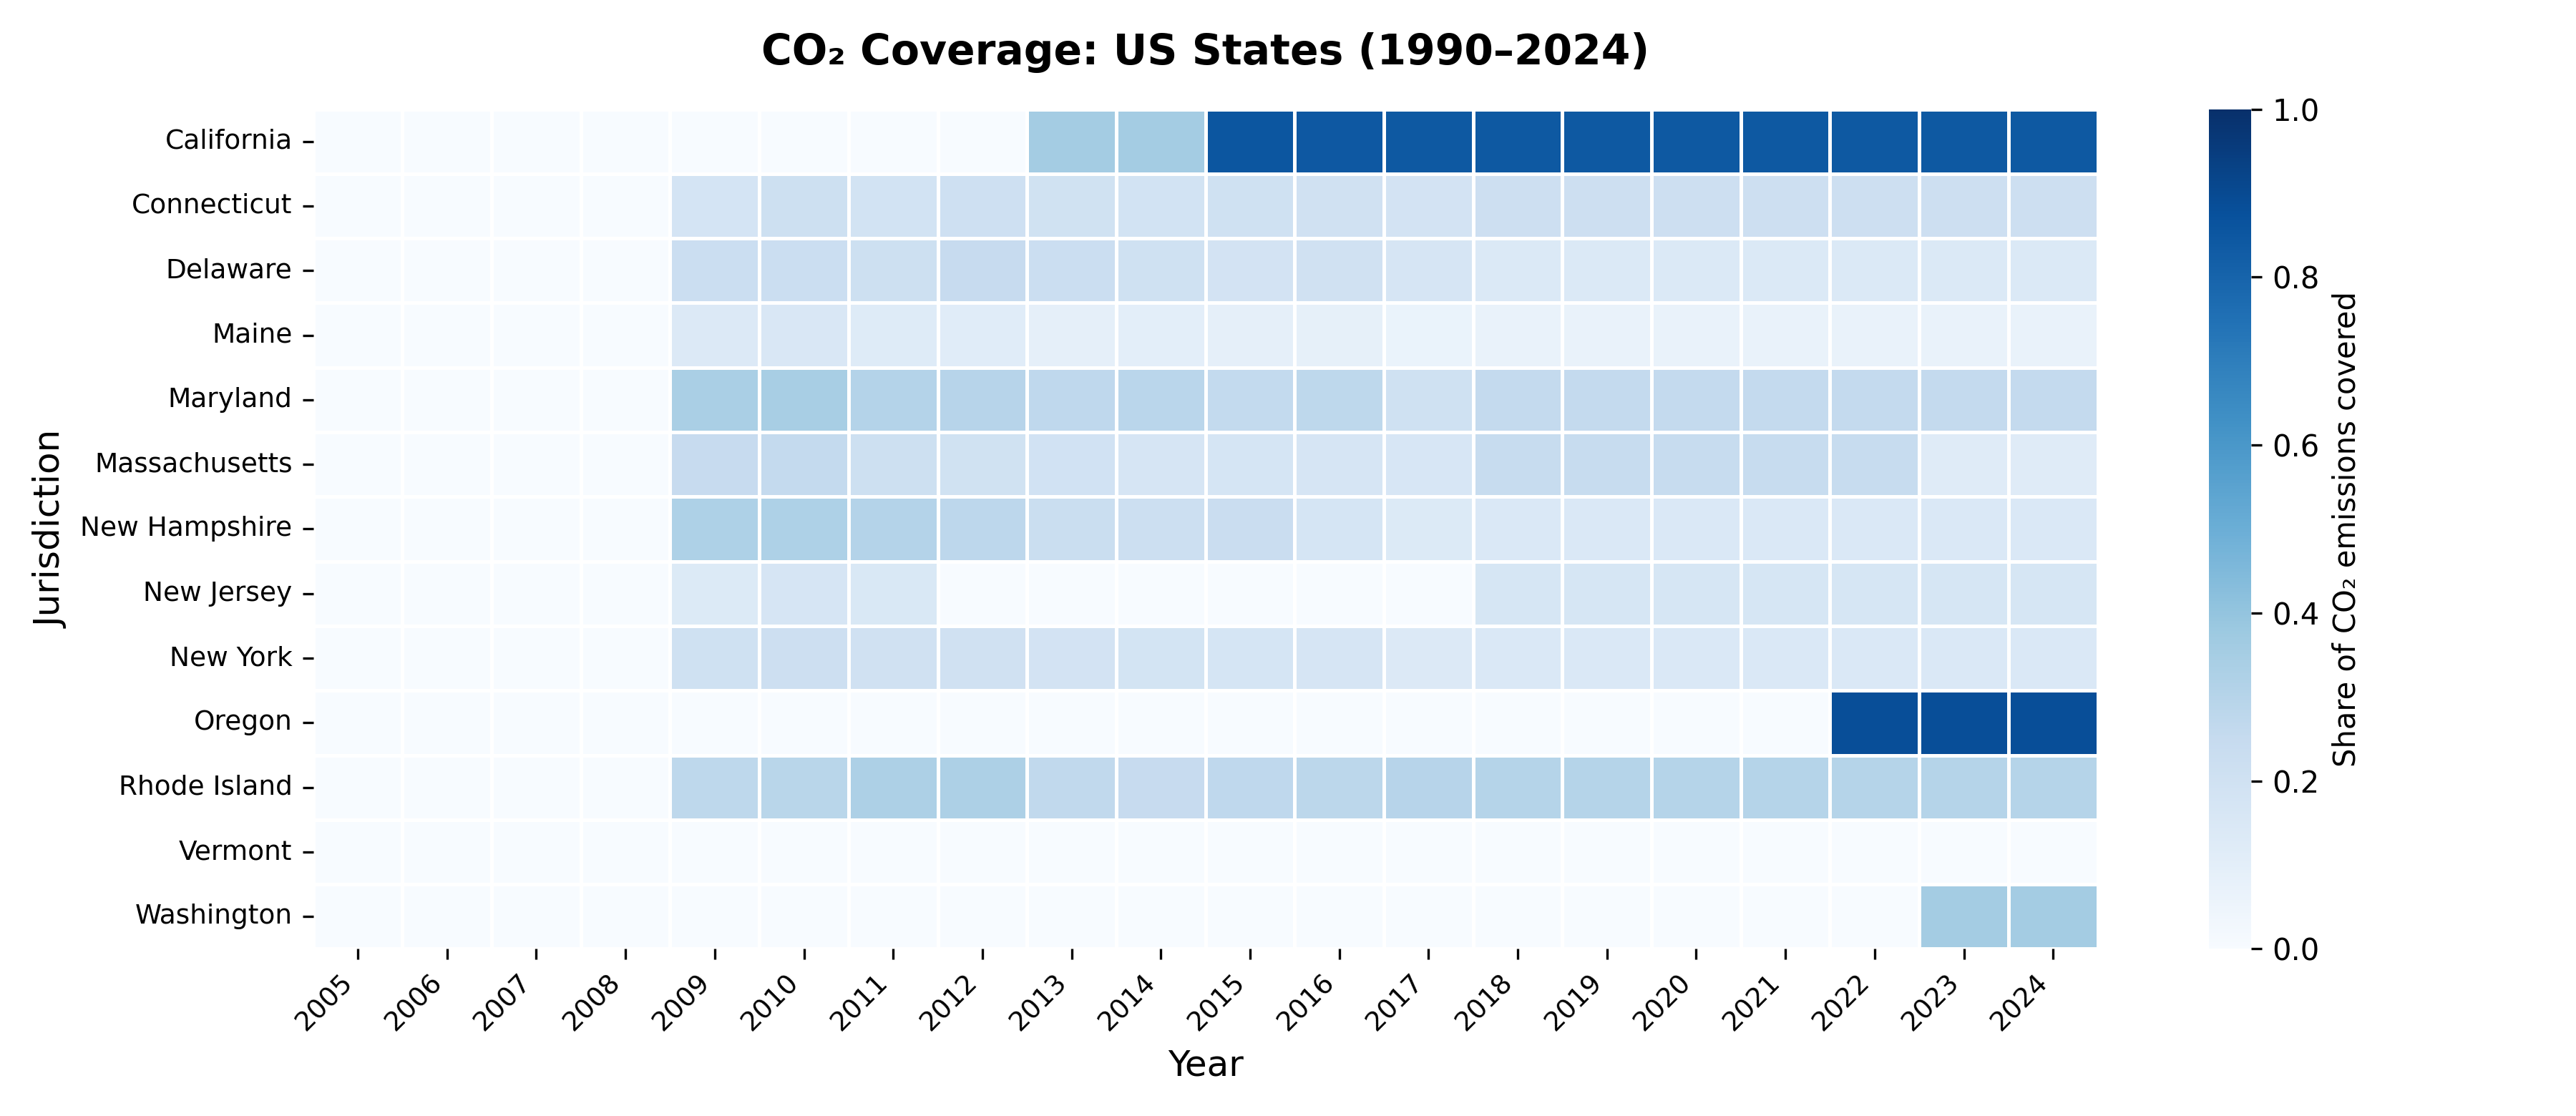
\includegraphics[keepaspectratio]{../../../_output/_figures/plots/coverage_hm_us.png}}

}

\caption{\label{fig-heatmap-coverage-us}Carbon pricing CO\(_2\) coverage
--- US States, 1990--2024}

\end{figure}%

\begin{figure}

\centering{

\pandocbounded{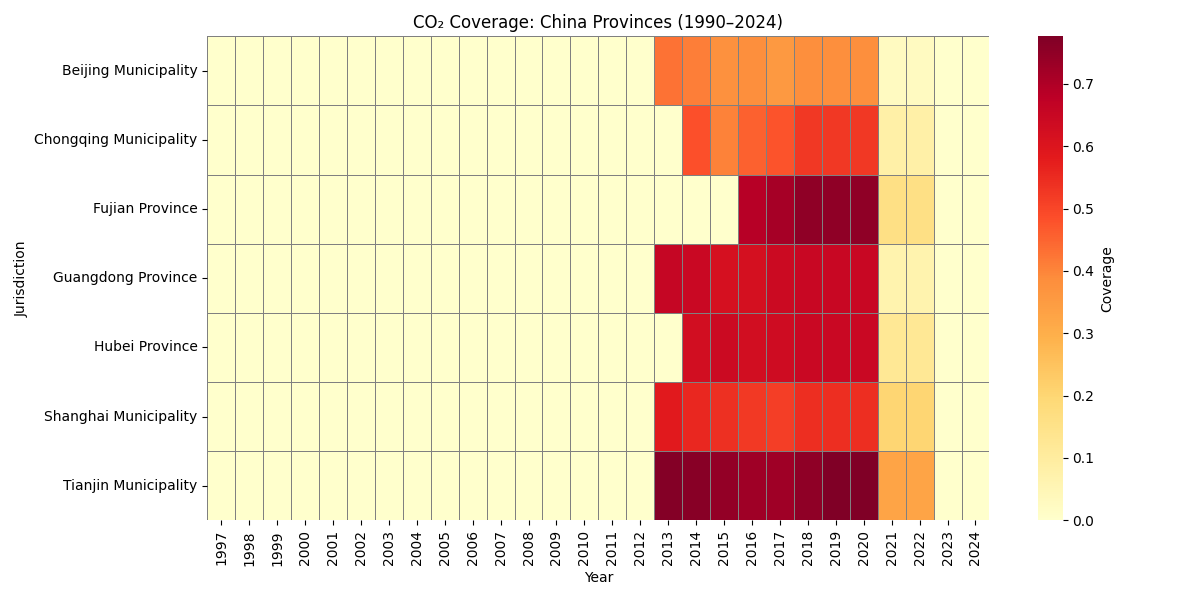
\includegraphics[keepaspectratio]{../../../_output/_figures/plots/coverage_hm_china.png}}

}

\caption{\label{fig-heatmap-coverage-china}Carbon pricing CO\(_2\)
coverage --- Chinese provinces, 1990--2024}

\end{figure}%

\begin{figure}

\centering{

\pandocbounded{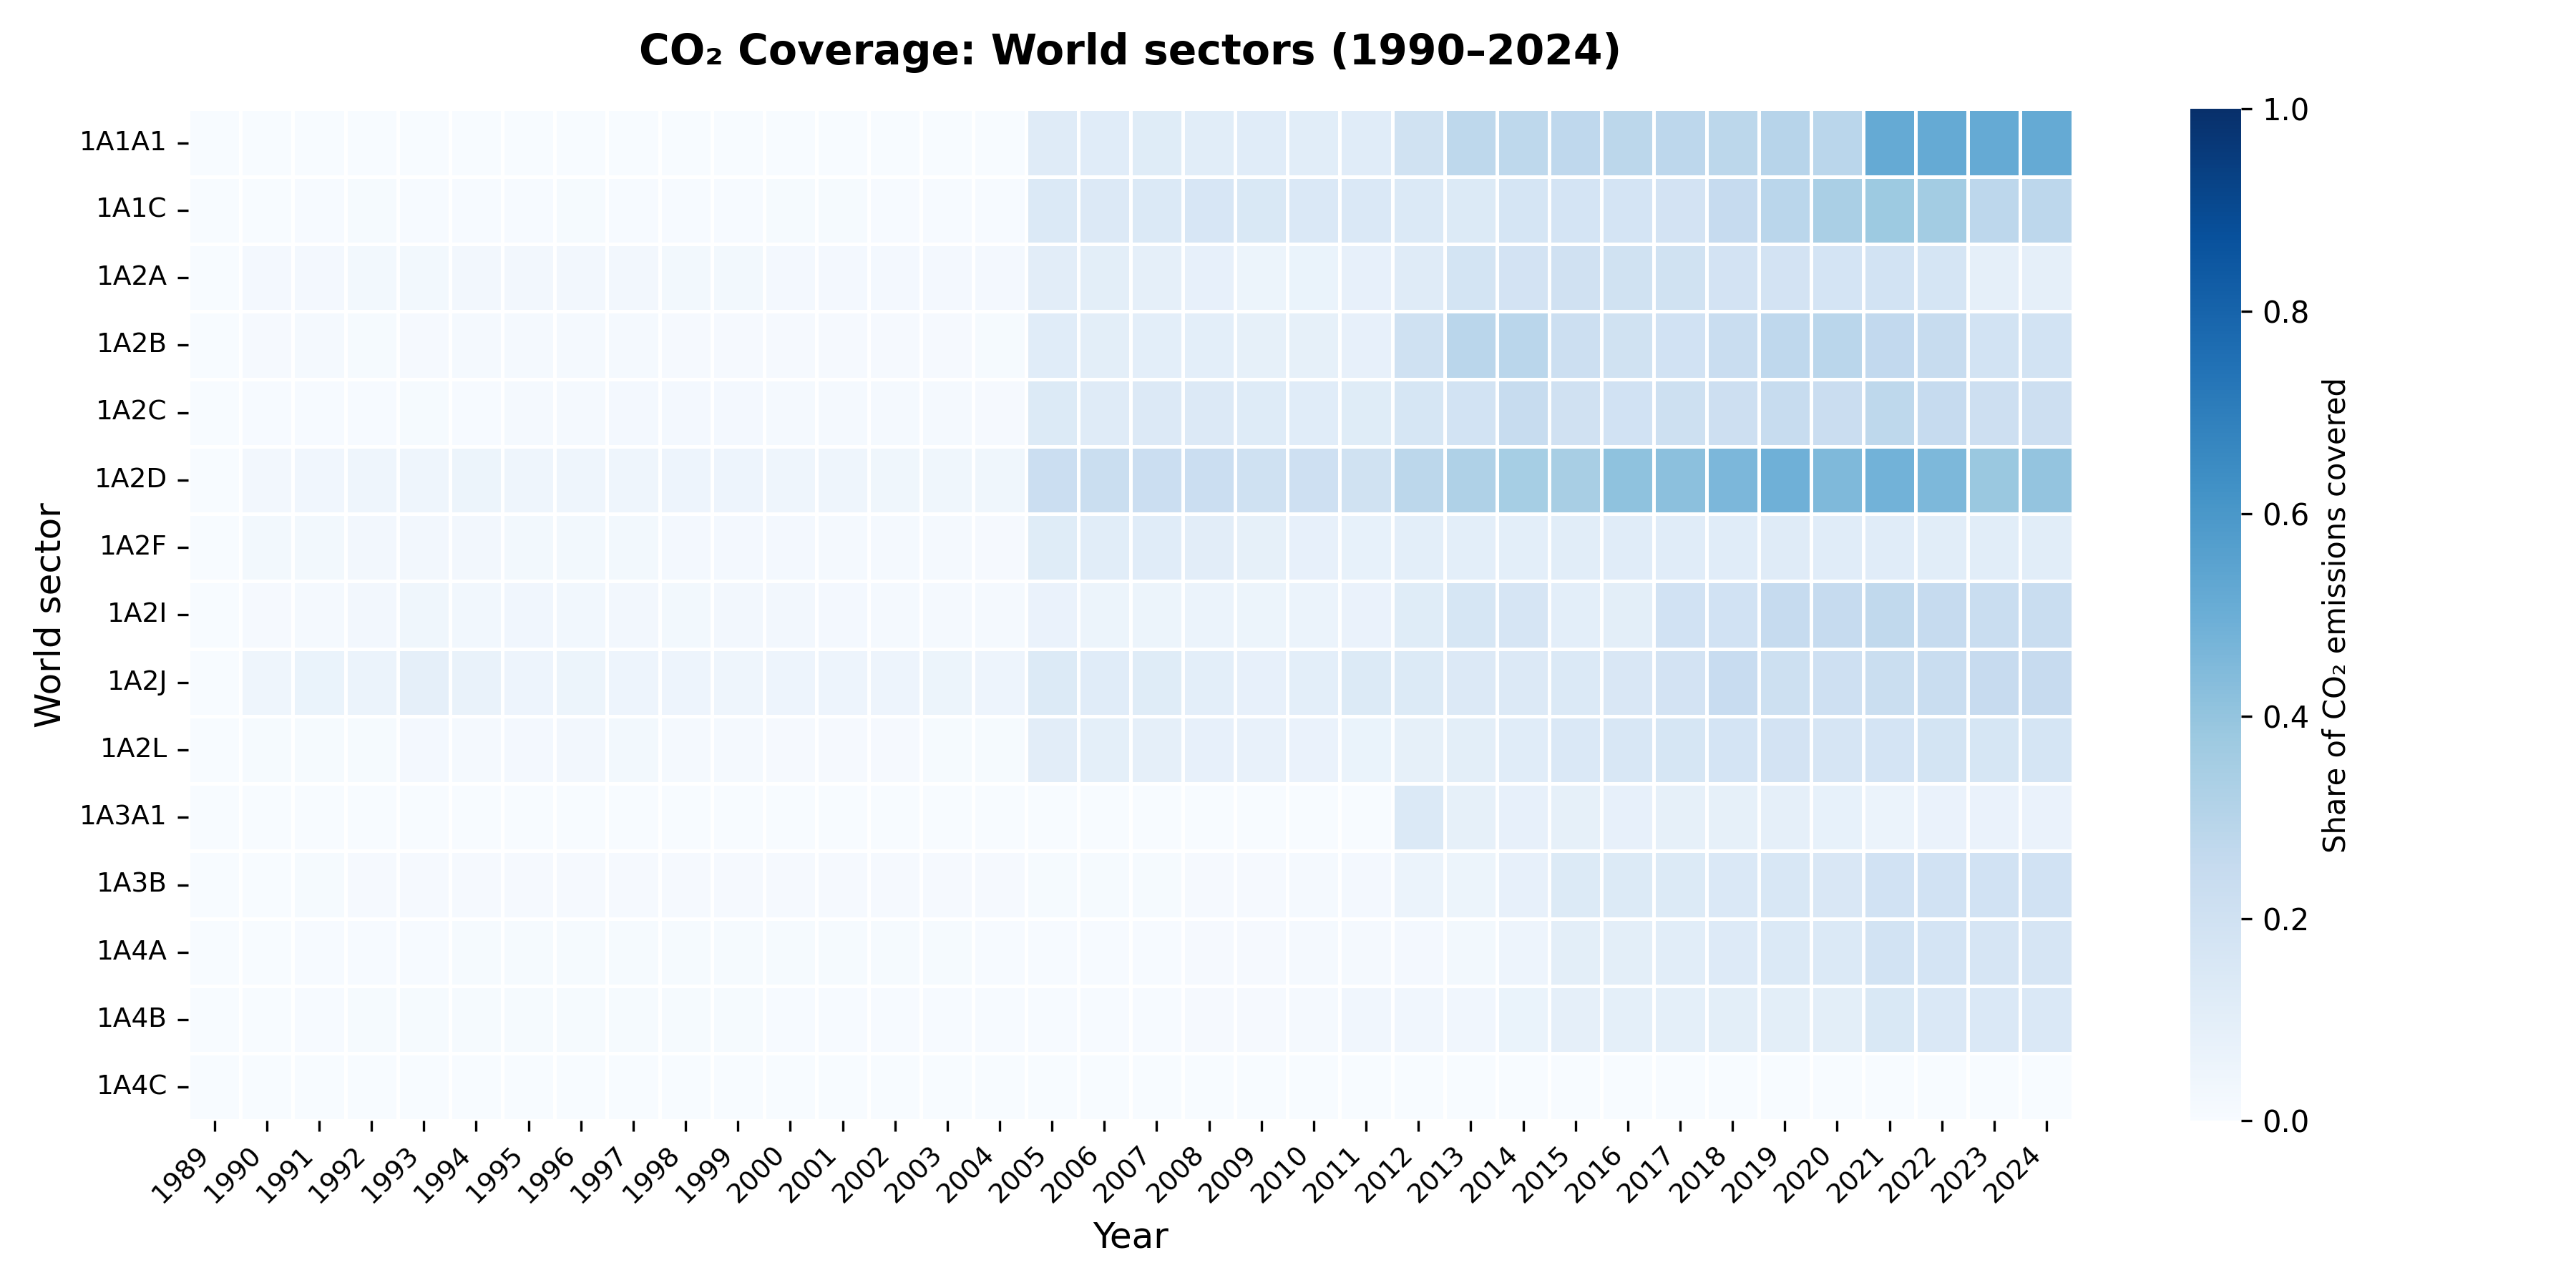
\includegraphics[keepaspectratio]{../../../_output/_figures/plots/coverage_hm_world_sec.png}}

}

\caption{\label{fig-heatmap-coverage-world_sec}Carbon pricing CO\(_2\)
coverage --- World sectors, 1990--2024}

\end{figure}%

\subsubsection{GDP}\label{gdp}

\begin{figure}

\centering{

\pandocbounded{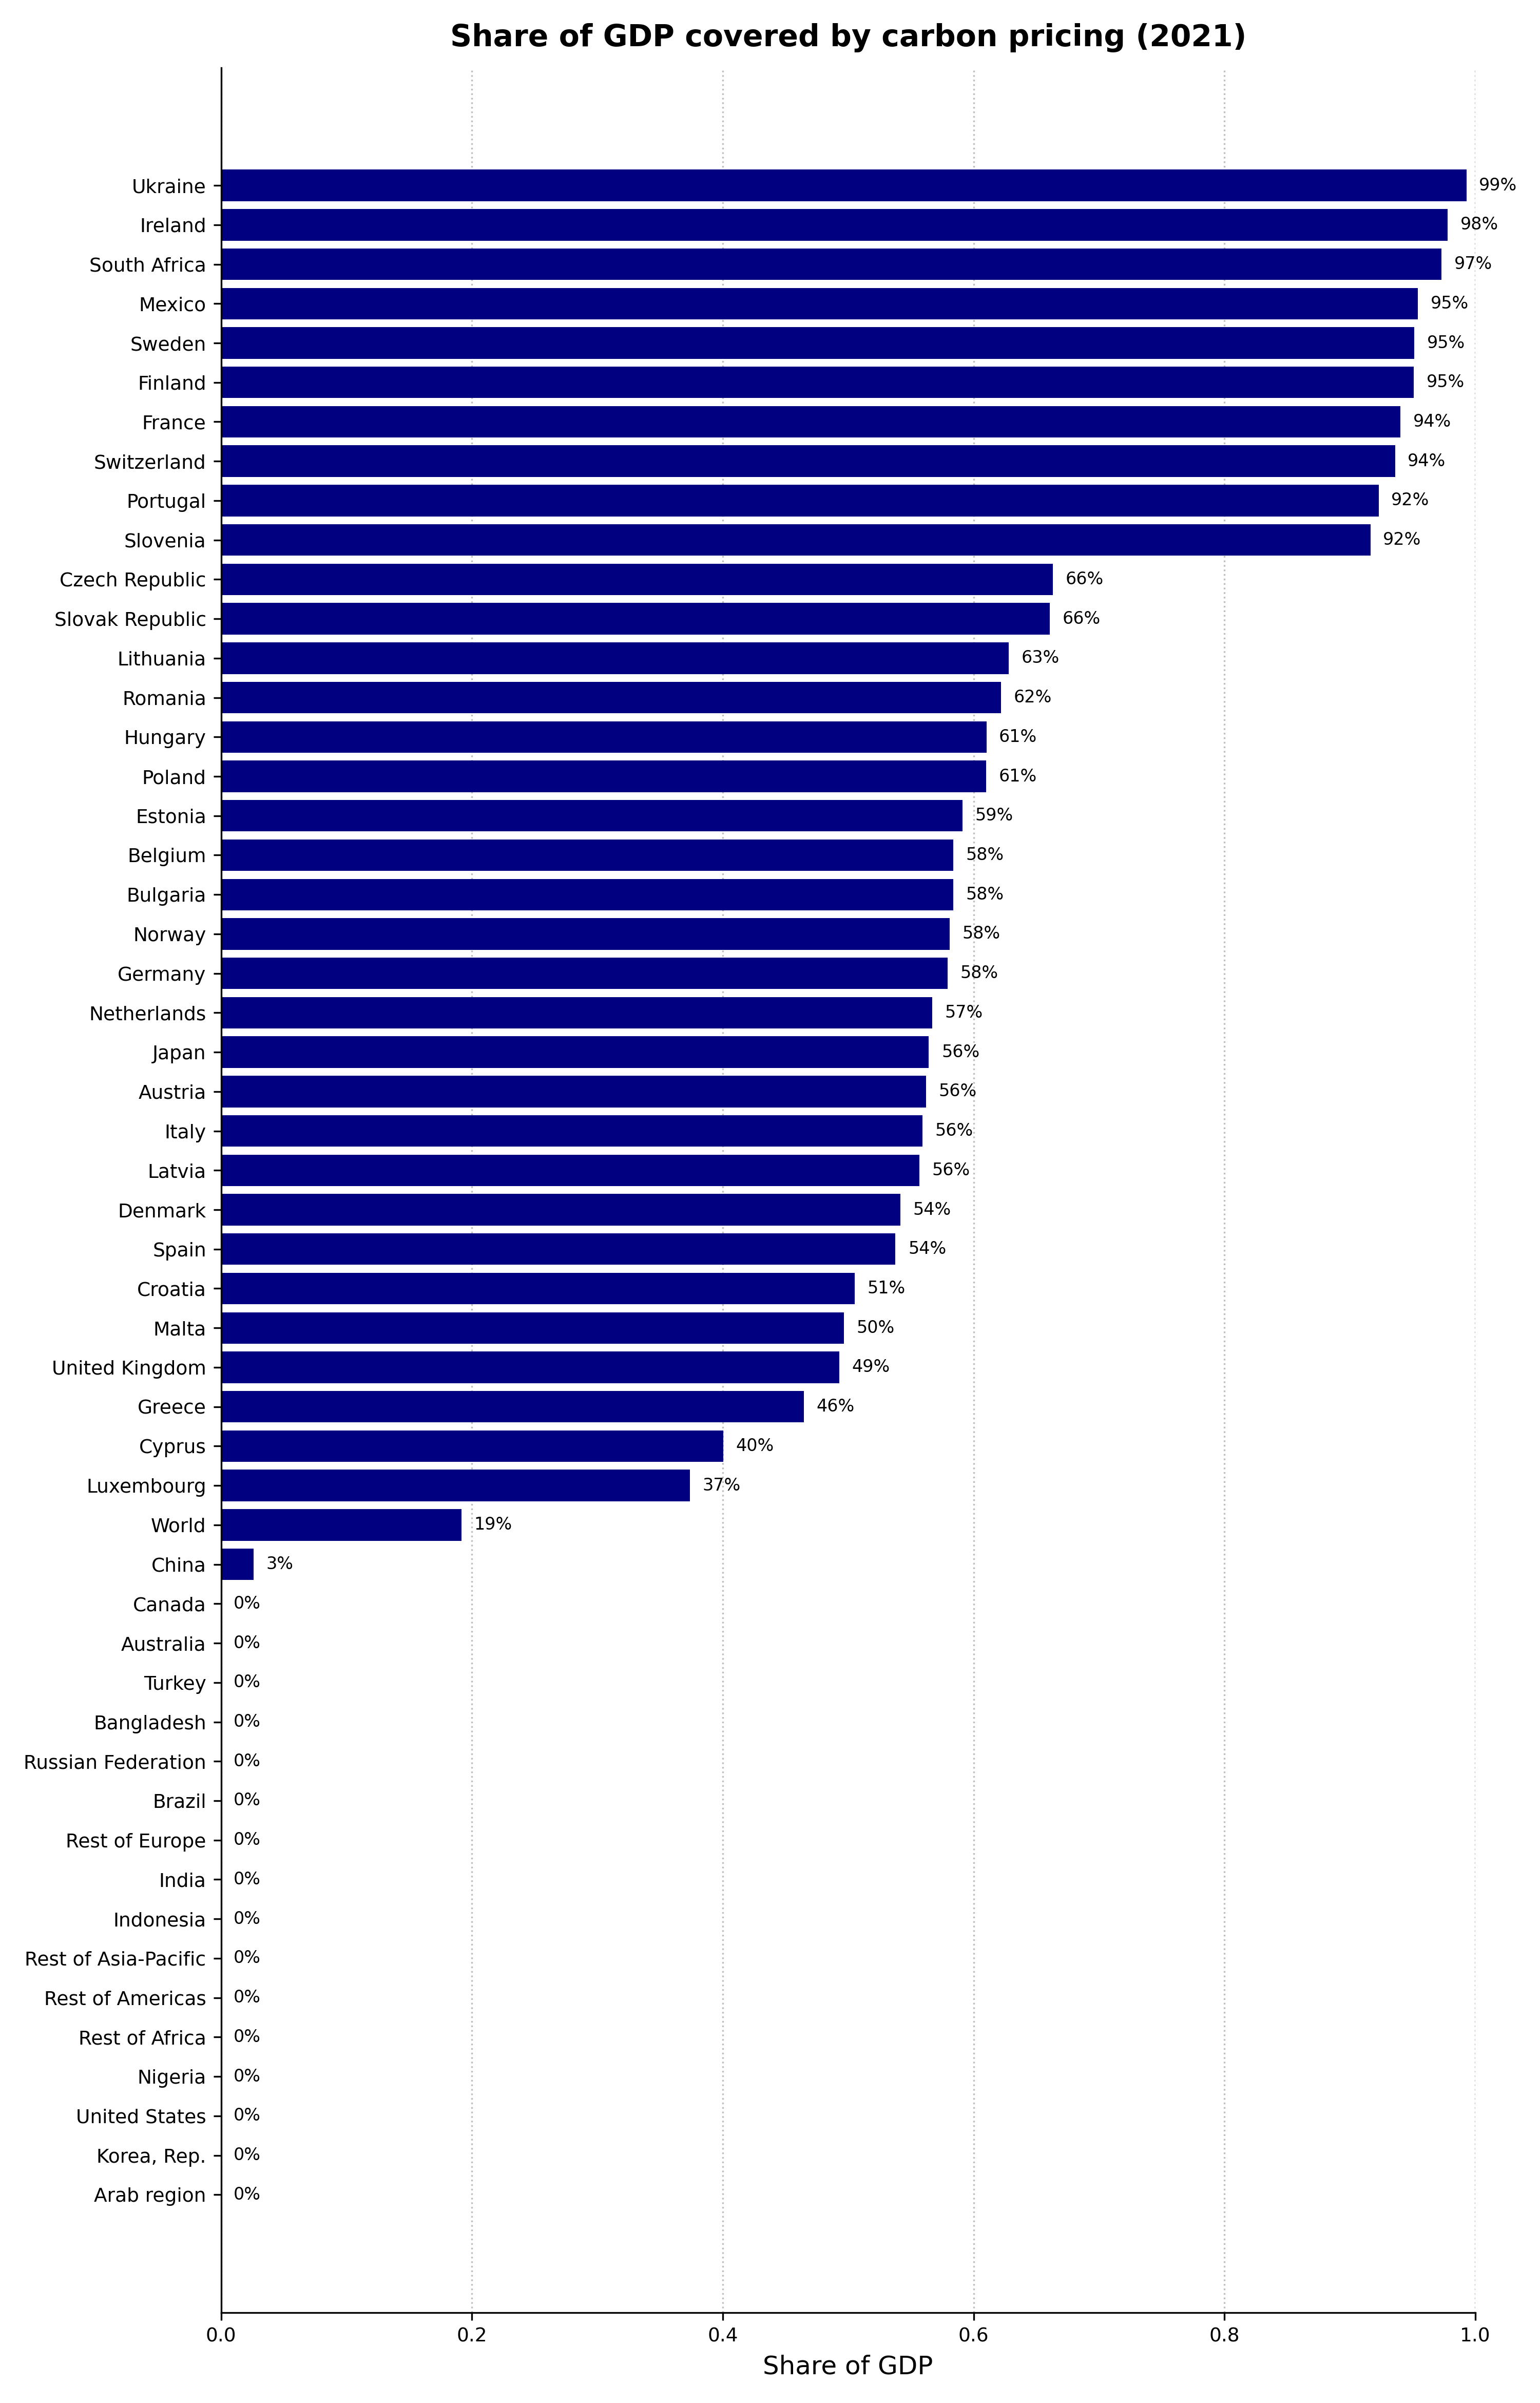
\includegraphics[keepaspectratio]{../../../_output/_figures/plots/gdp_coverage_bar.png}}

}

\caption{\label{fig-bar-coverage-gdp}Carbon pricing GDP coverage -
countries, 1990--2024}

\end{figure}%

\newpage

\subsection{Prices}\label{prices}

\begin{figure}

\centering{

\pandocbounded{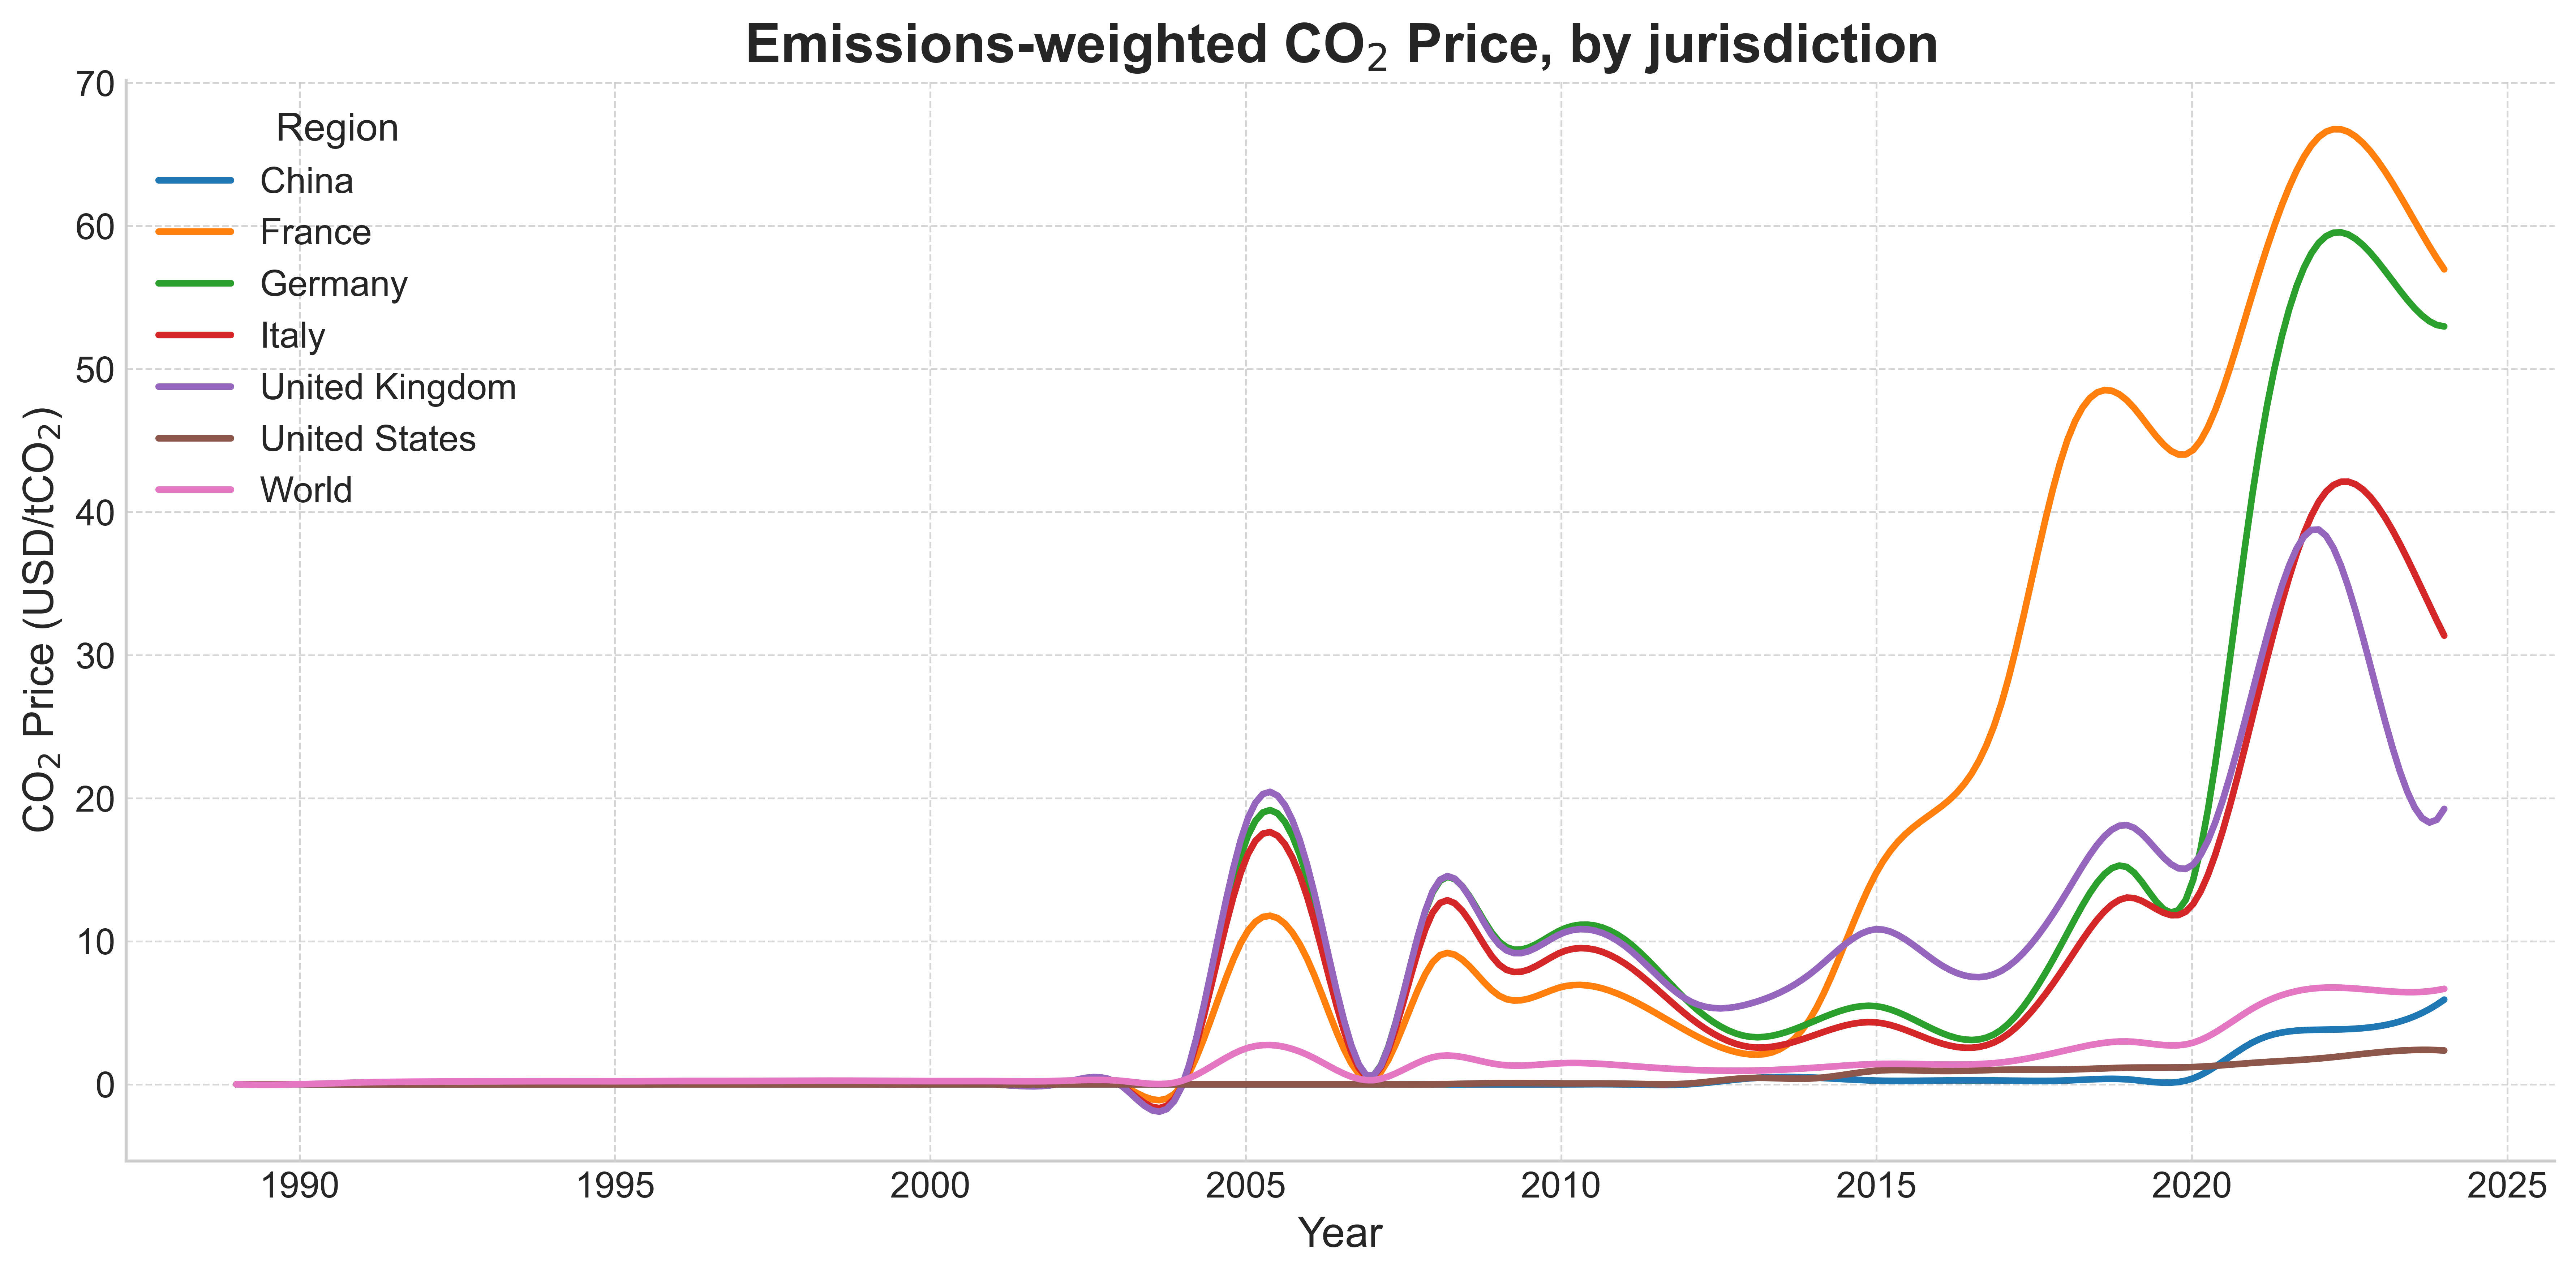
\includegraphics[keepaspectratio]{../../../_output/_figures/plots/ecp_co2_ts.png}}

}

\caption{\label{fig-ecp-ts}Average carbon price by country, 1990--2024}

\end{figure}%

\begin{figure}

\centering{

\pandocbounded{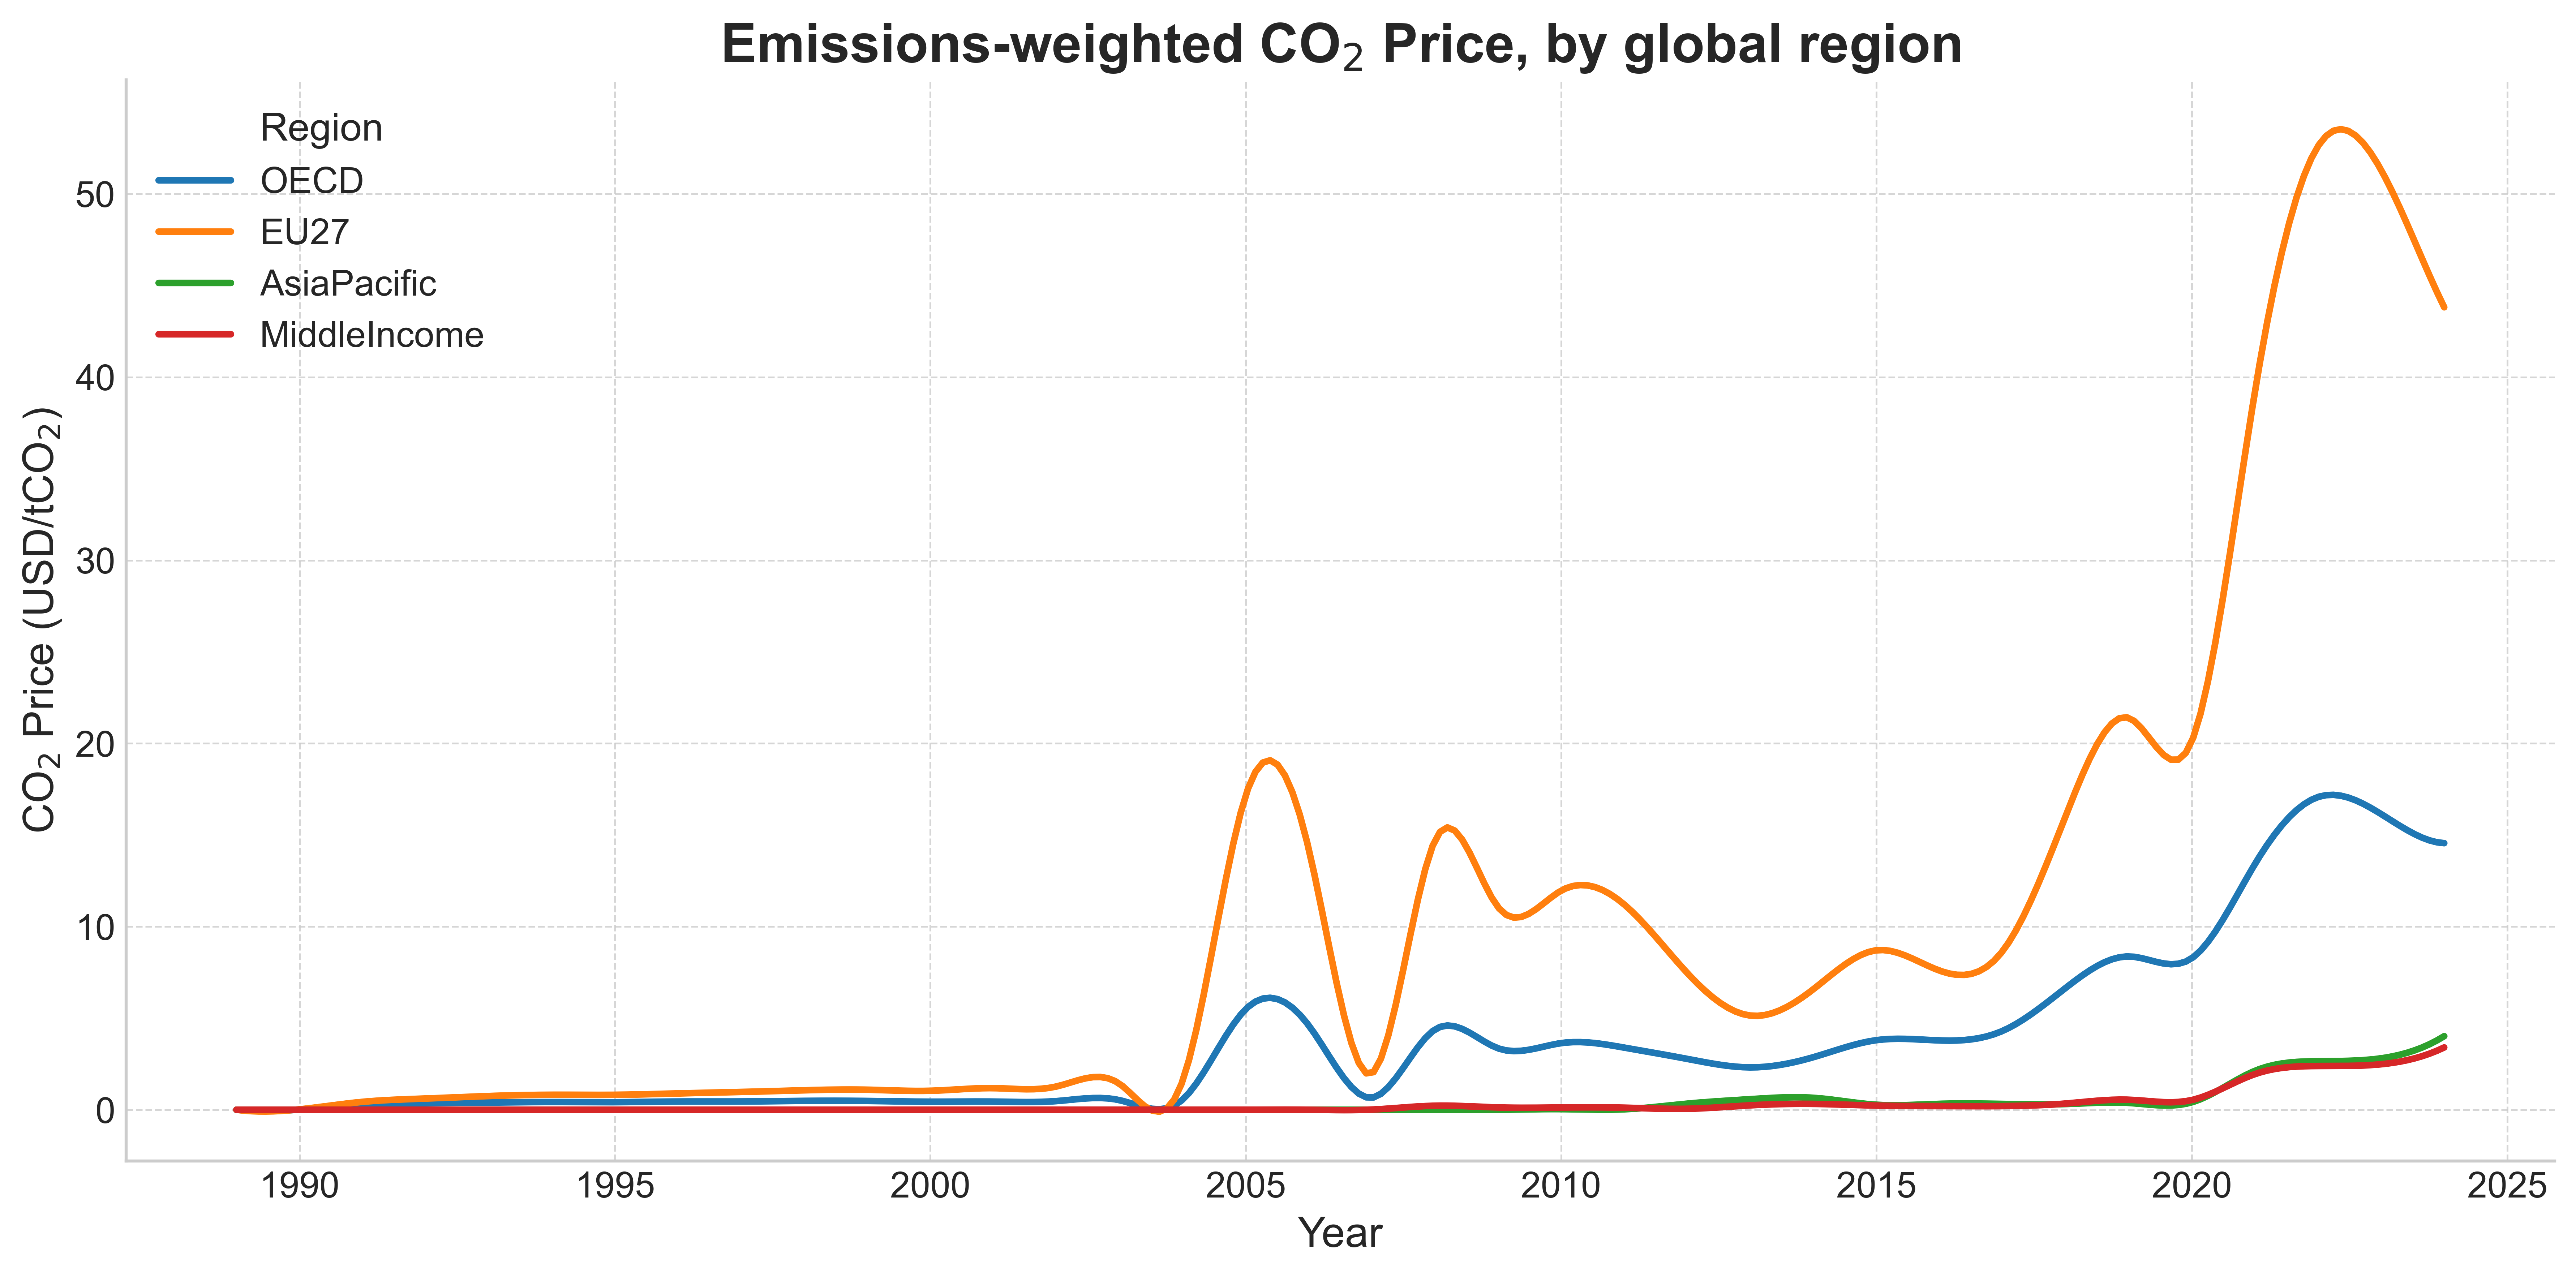
\includegraphics[keepaspectratio]{../../../_output/_figures/plots/ecp_co2_regional.png}}

}

\caption{\label{fig-ecp-region}Average carbon price by global region,
1990--2024}

\end{figure}%

\begin{figure}

\centering{

\pandocbounded{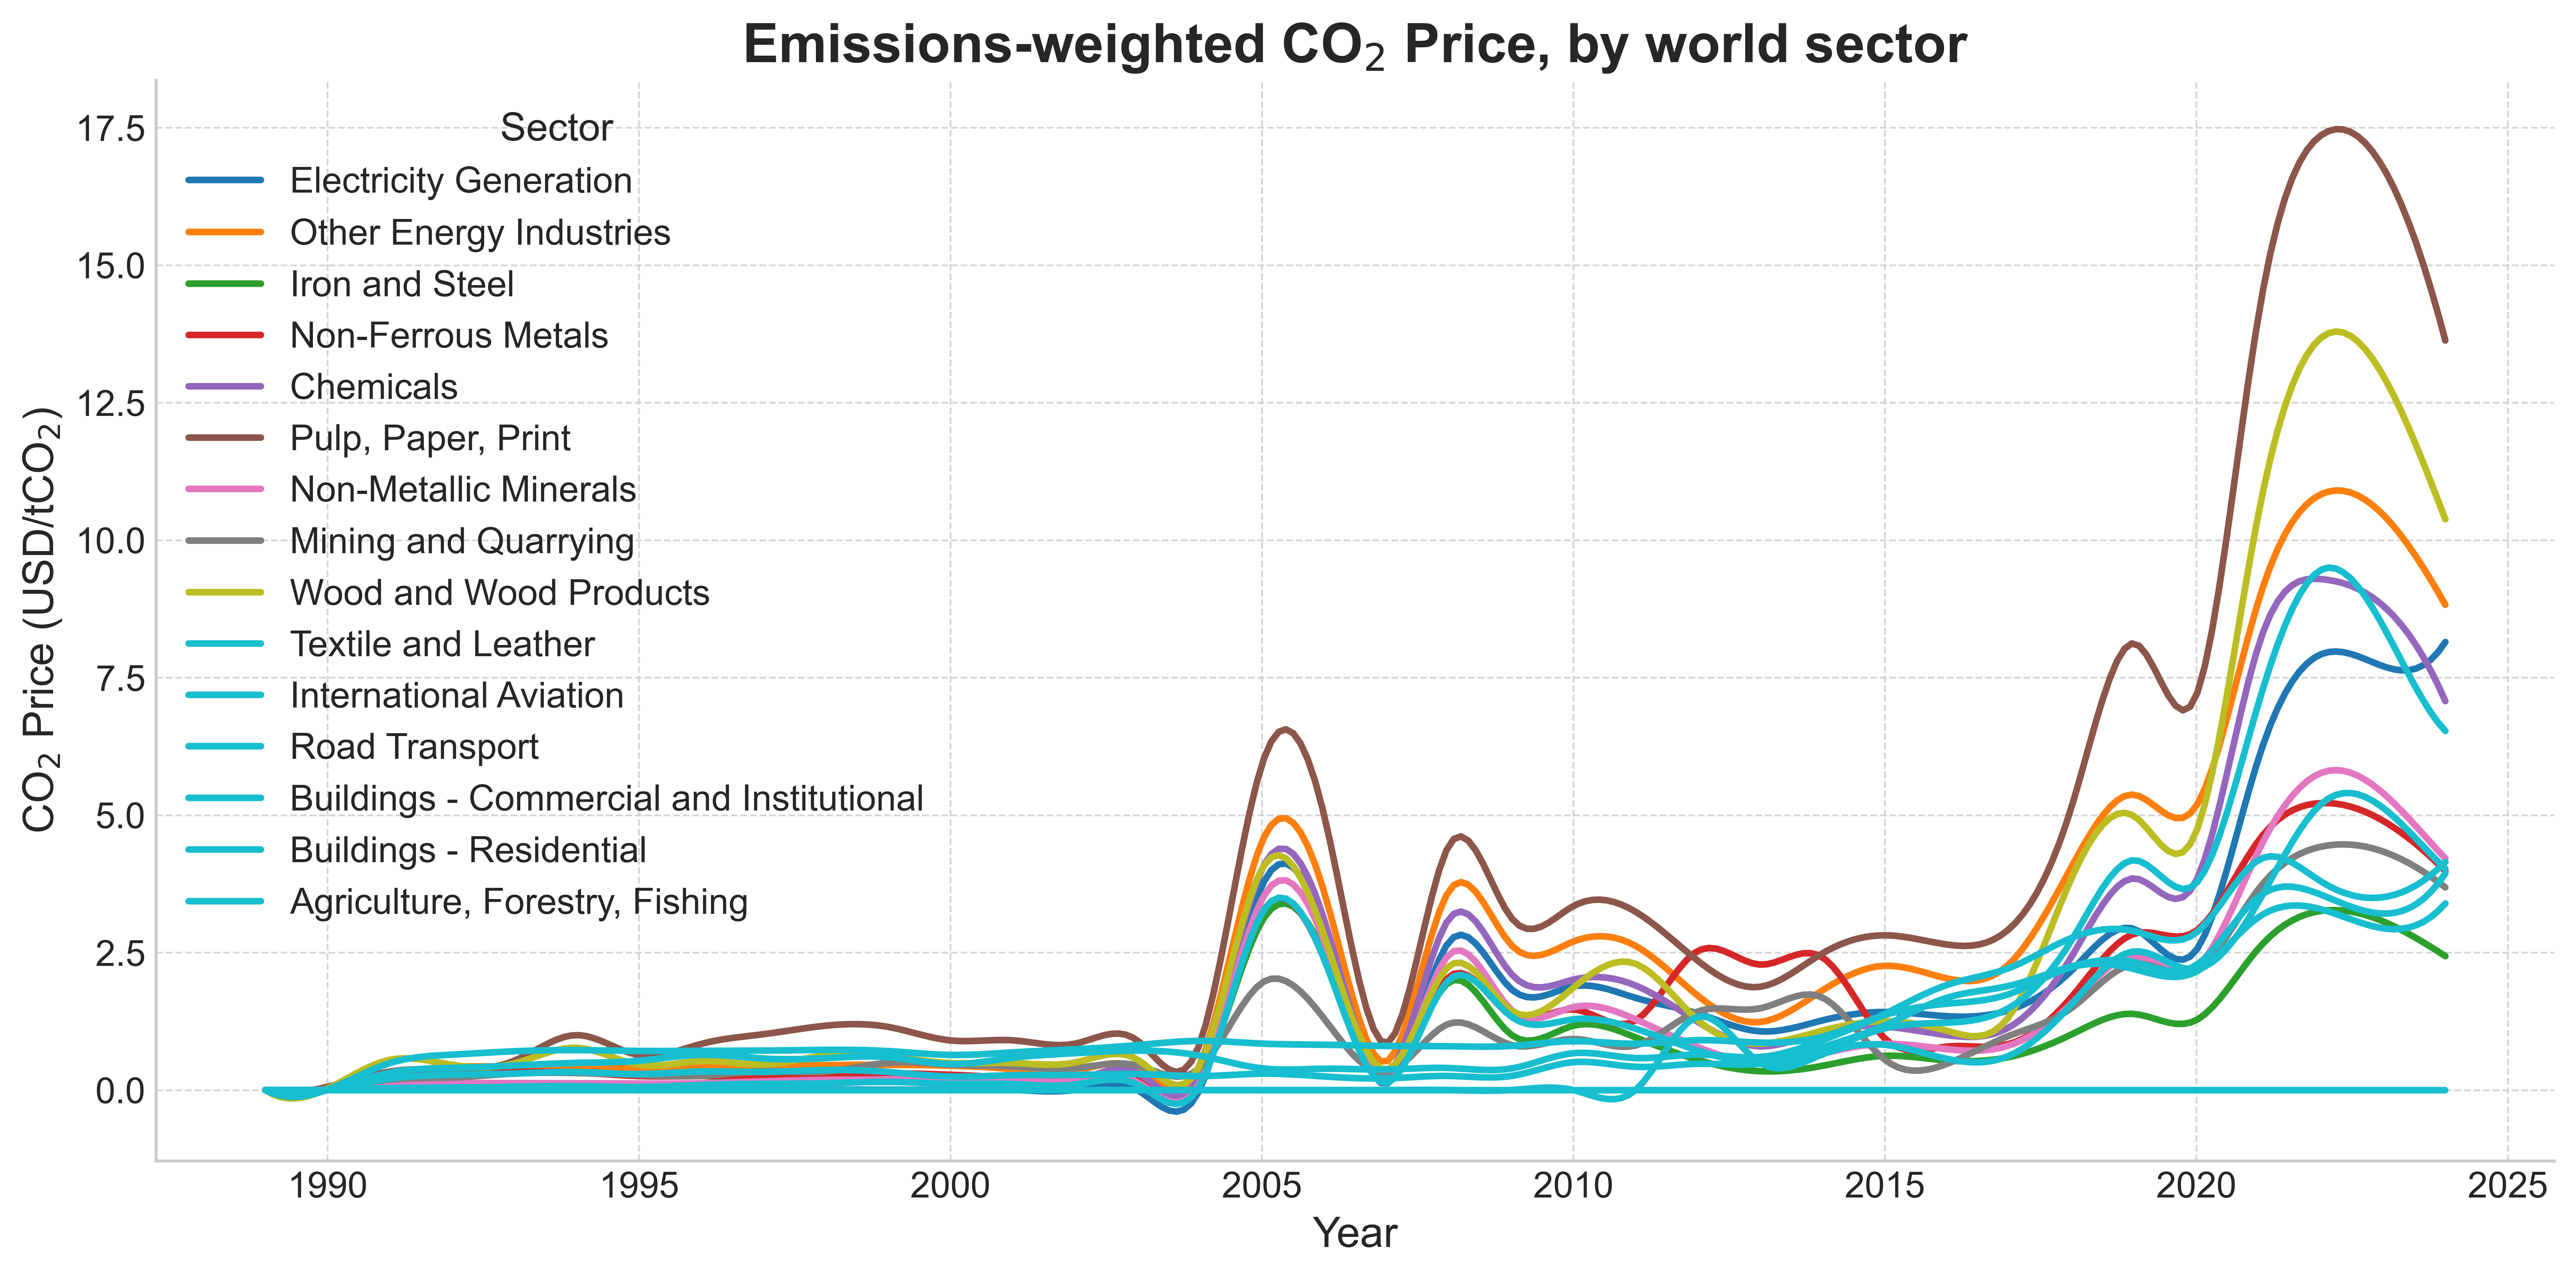
\includegraphics[keepaspectratio]{../../../_output/_figures/plots/ecp_co2_ts_world_sec.png}}

}

\caption{\label{fig-ecp-world-sec}Average carbon price by global sector,
1990--2024}

\end{figure}%

\begin{figure}

\centering{

\pandocbounded{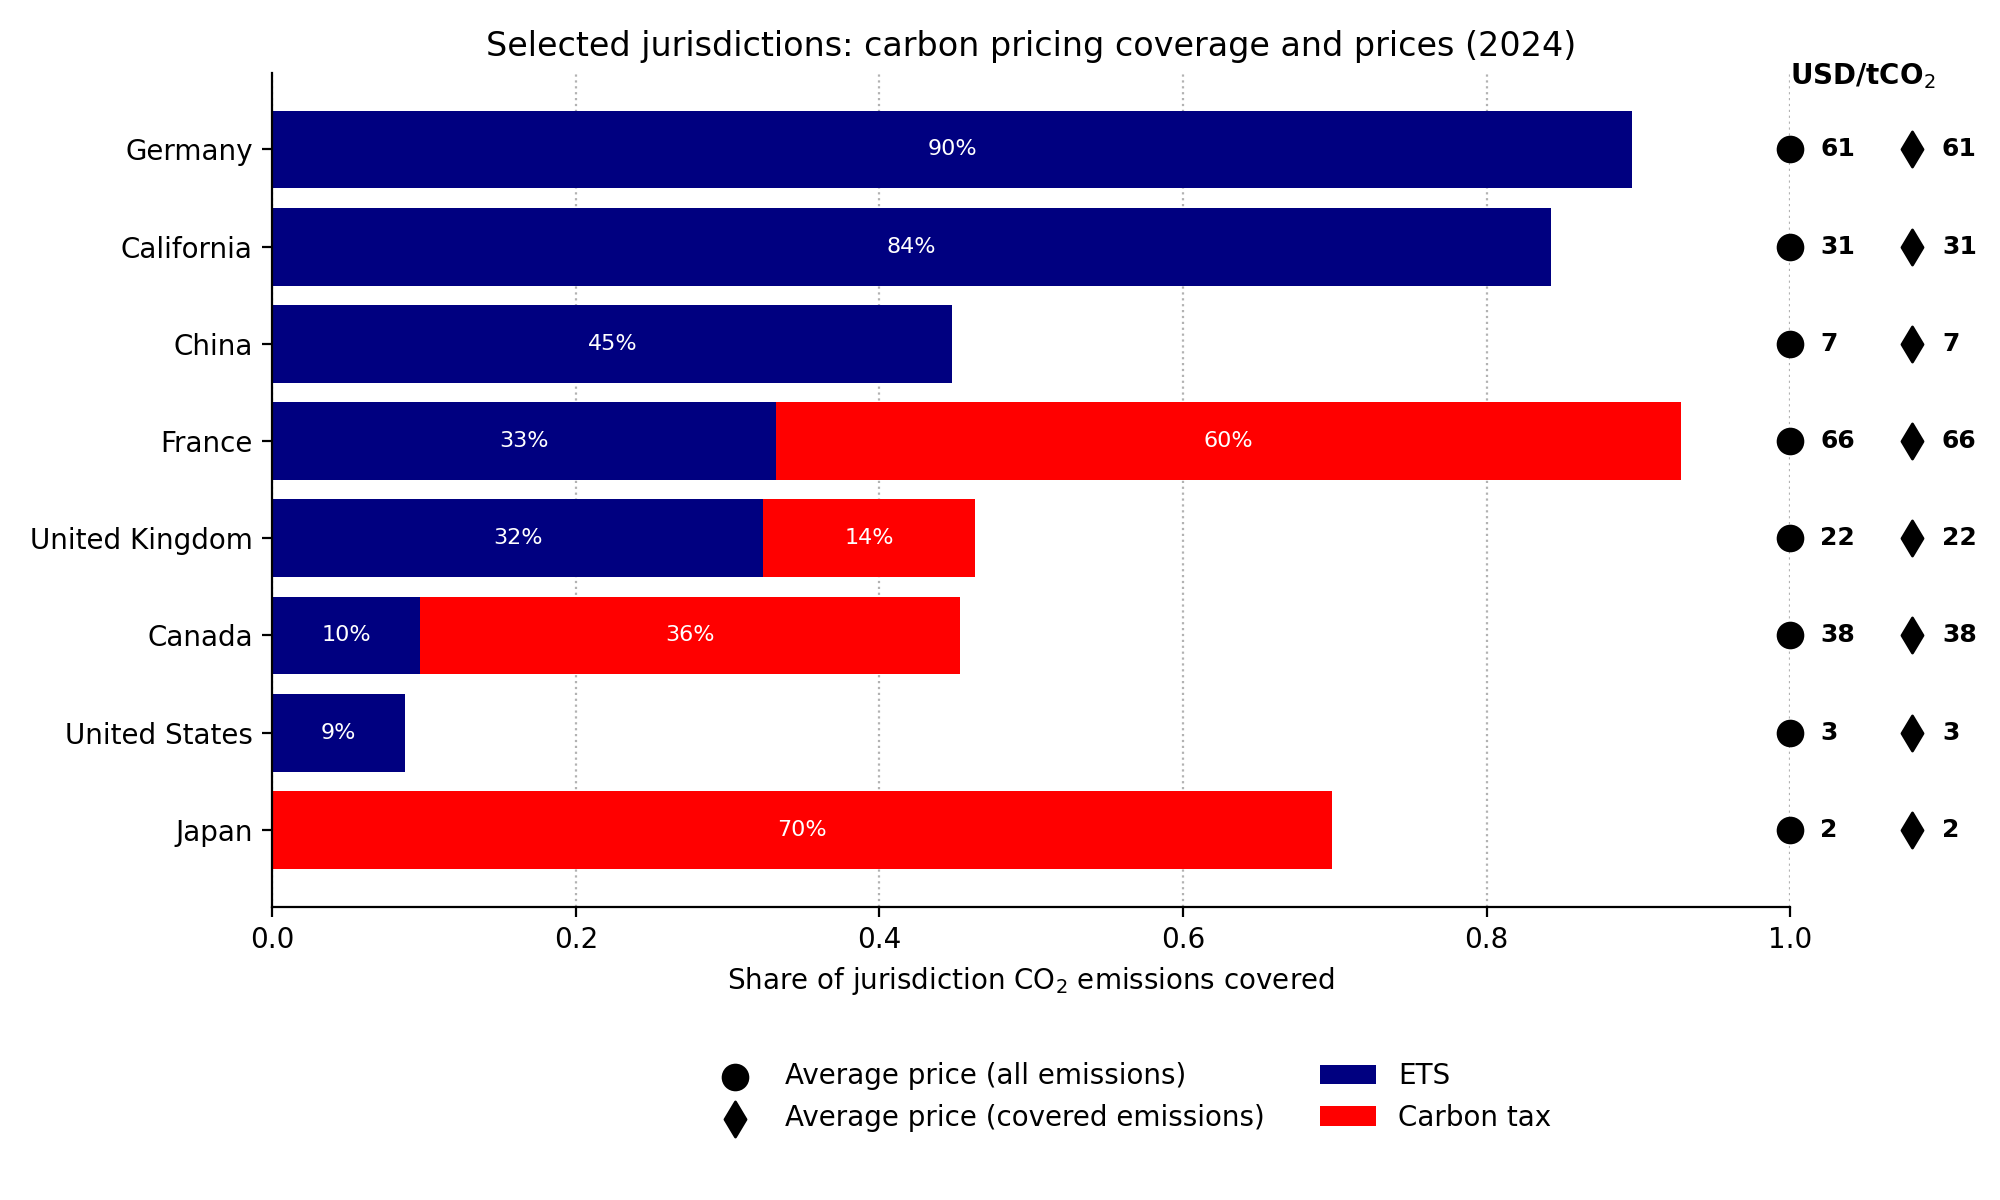
\includegraphics[keepaspectratio]{../../../_output/_figures/plots/selected_jurisdictions_ecp.png}}

}

\caption{\label{fig-ecp-ets-tax}Carbon pricing CO\(_2\) coverage and
prices, 2024}

\end{figure}%

\begin{figure}

\centering{

\pandocbounded{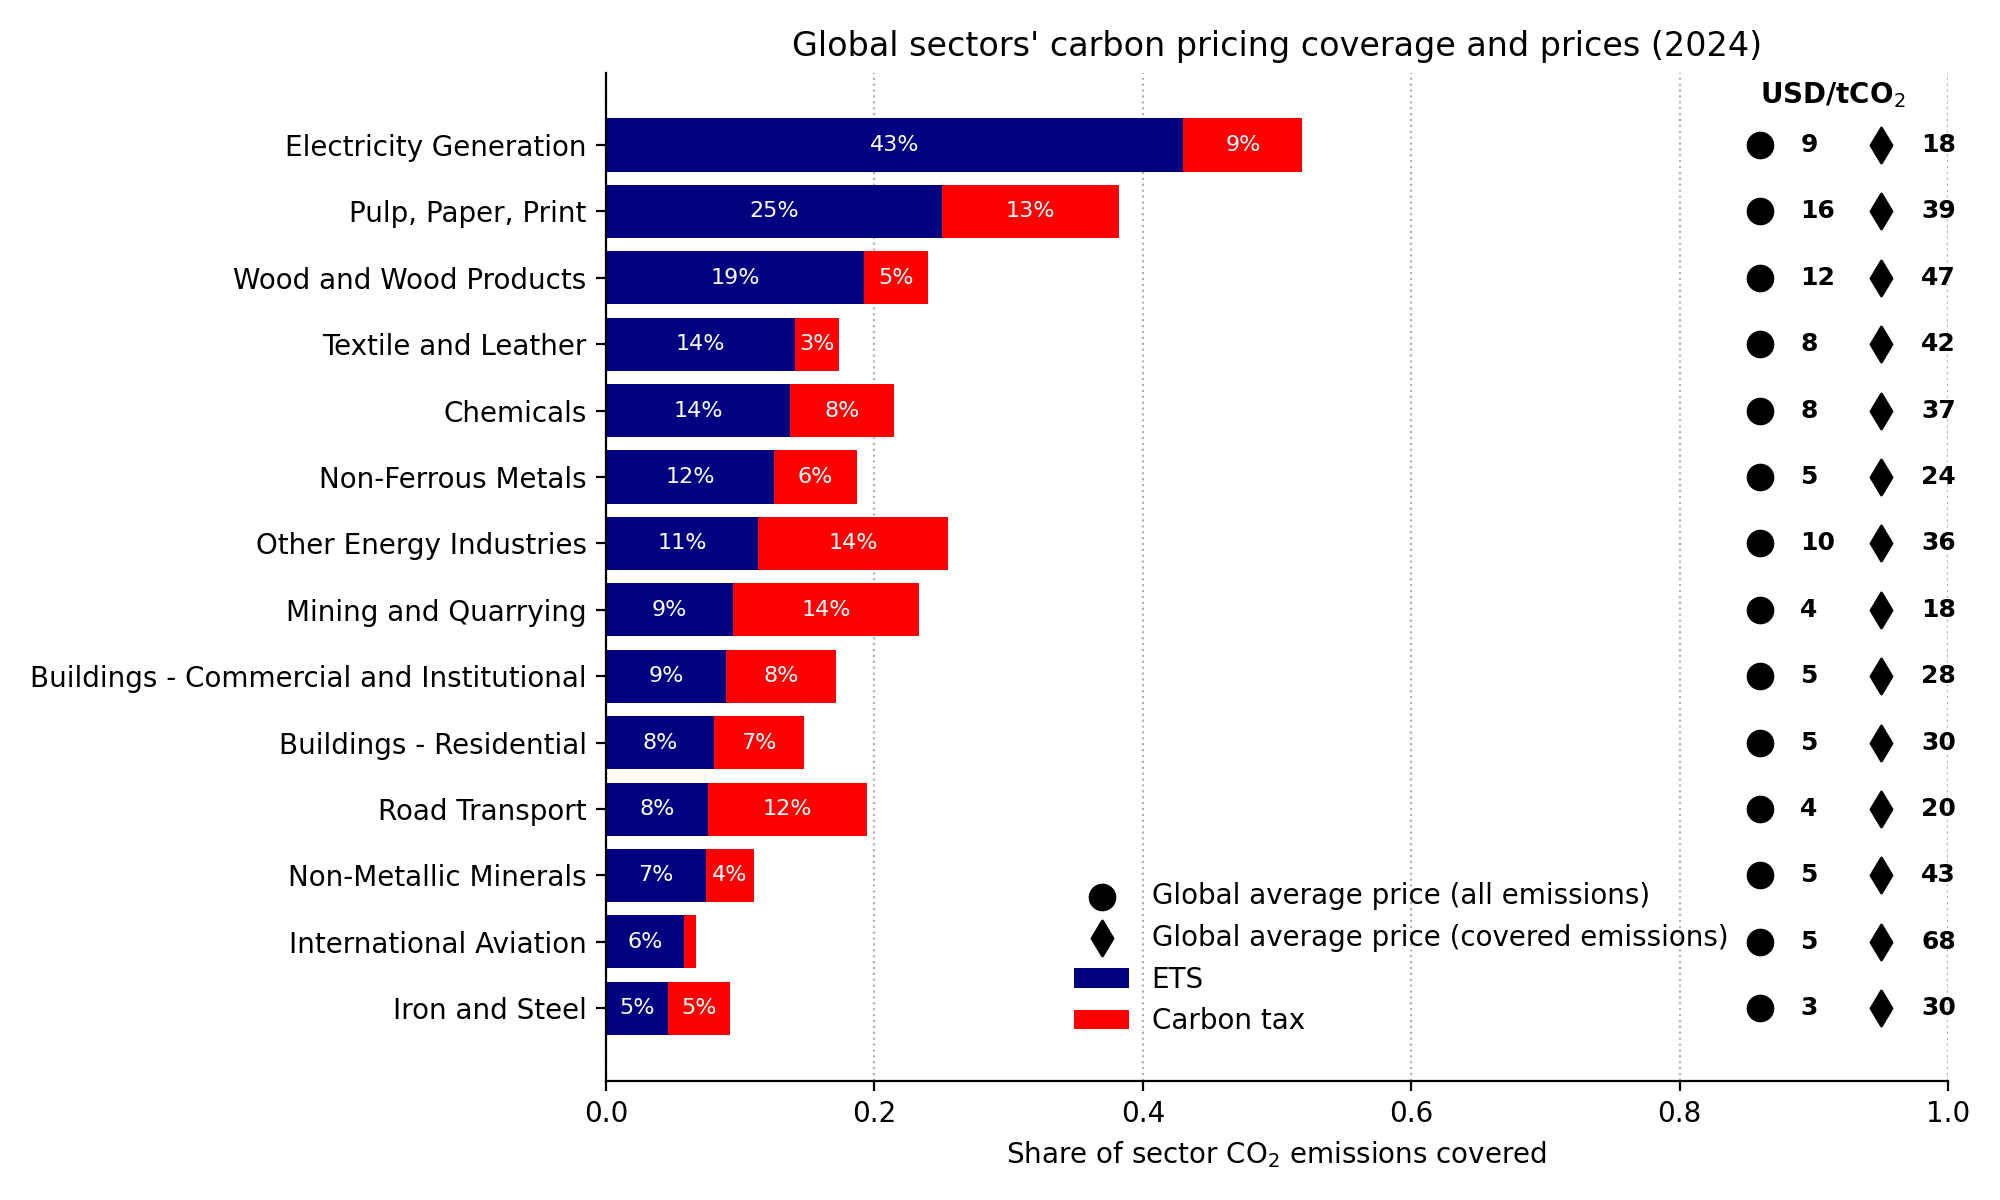
\includegraphics[keepaspectratio]{../../../_output/_figures/plots/world_sectors_ecp.png}}

}

\caption{\label{fig-ecp_coverage-world_sectors}Average carbon prices and
CO\(_2\) coverage by world sectors, 2024}

\end{figure}%

\begin{figure}

\centering{

\pandocbounded{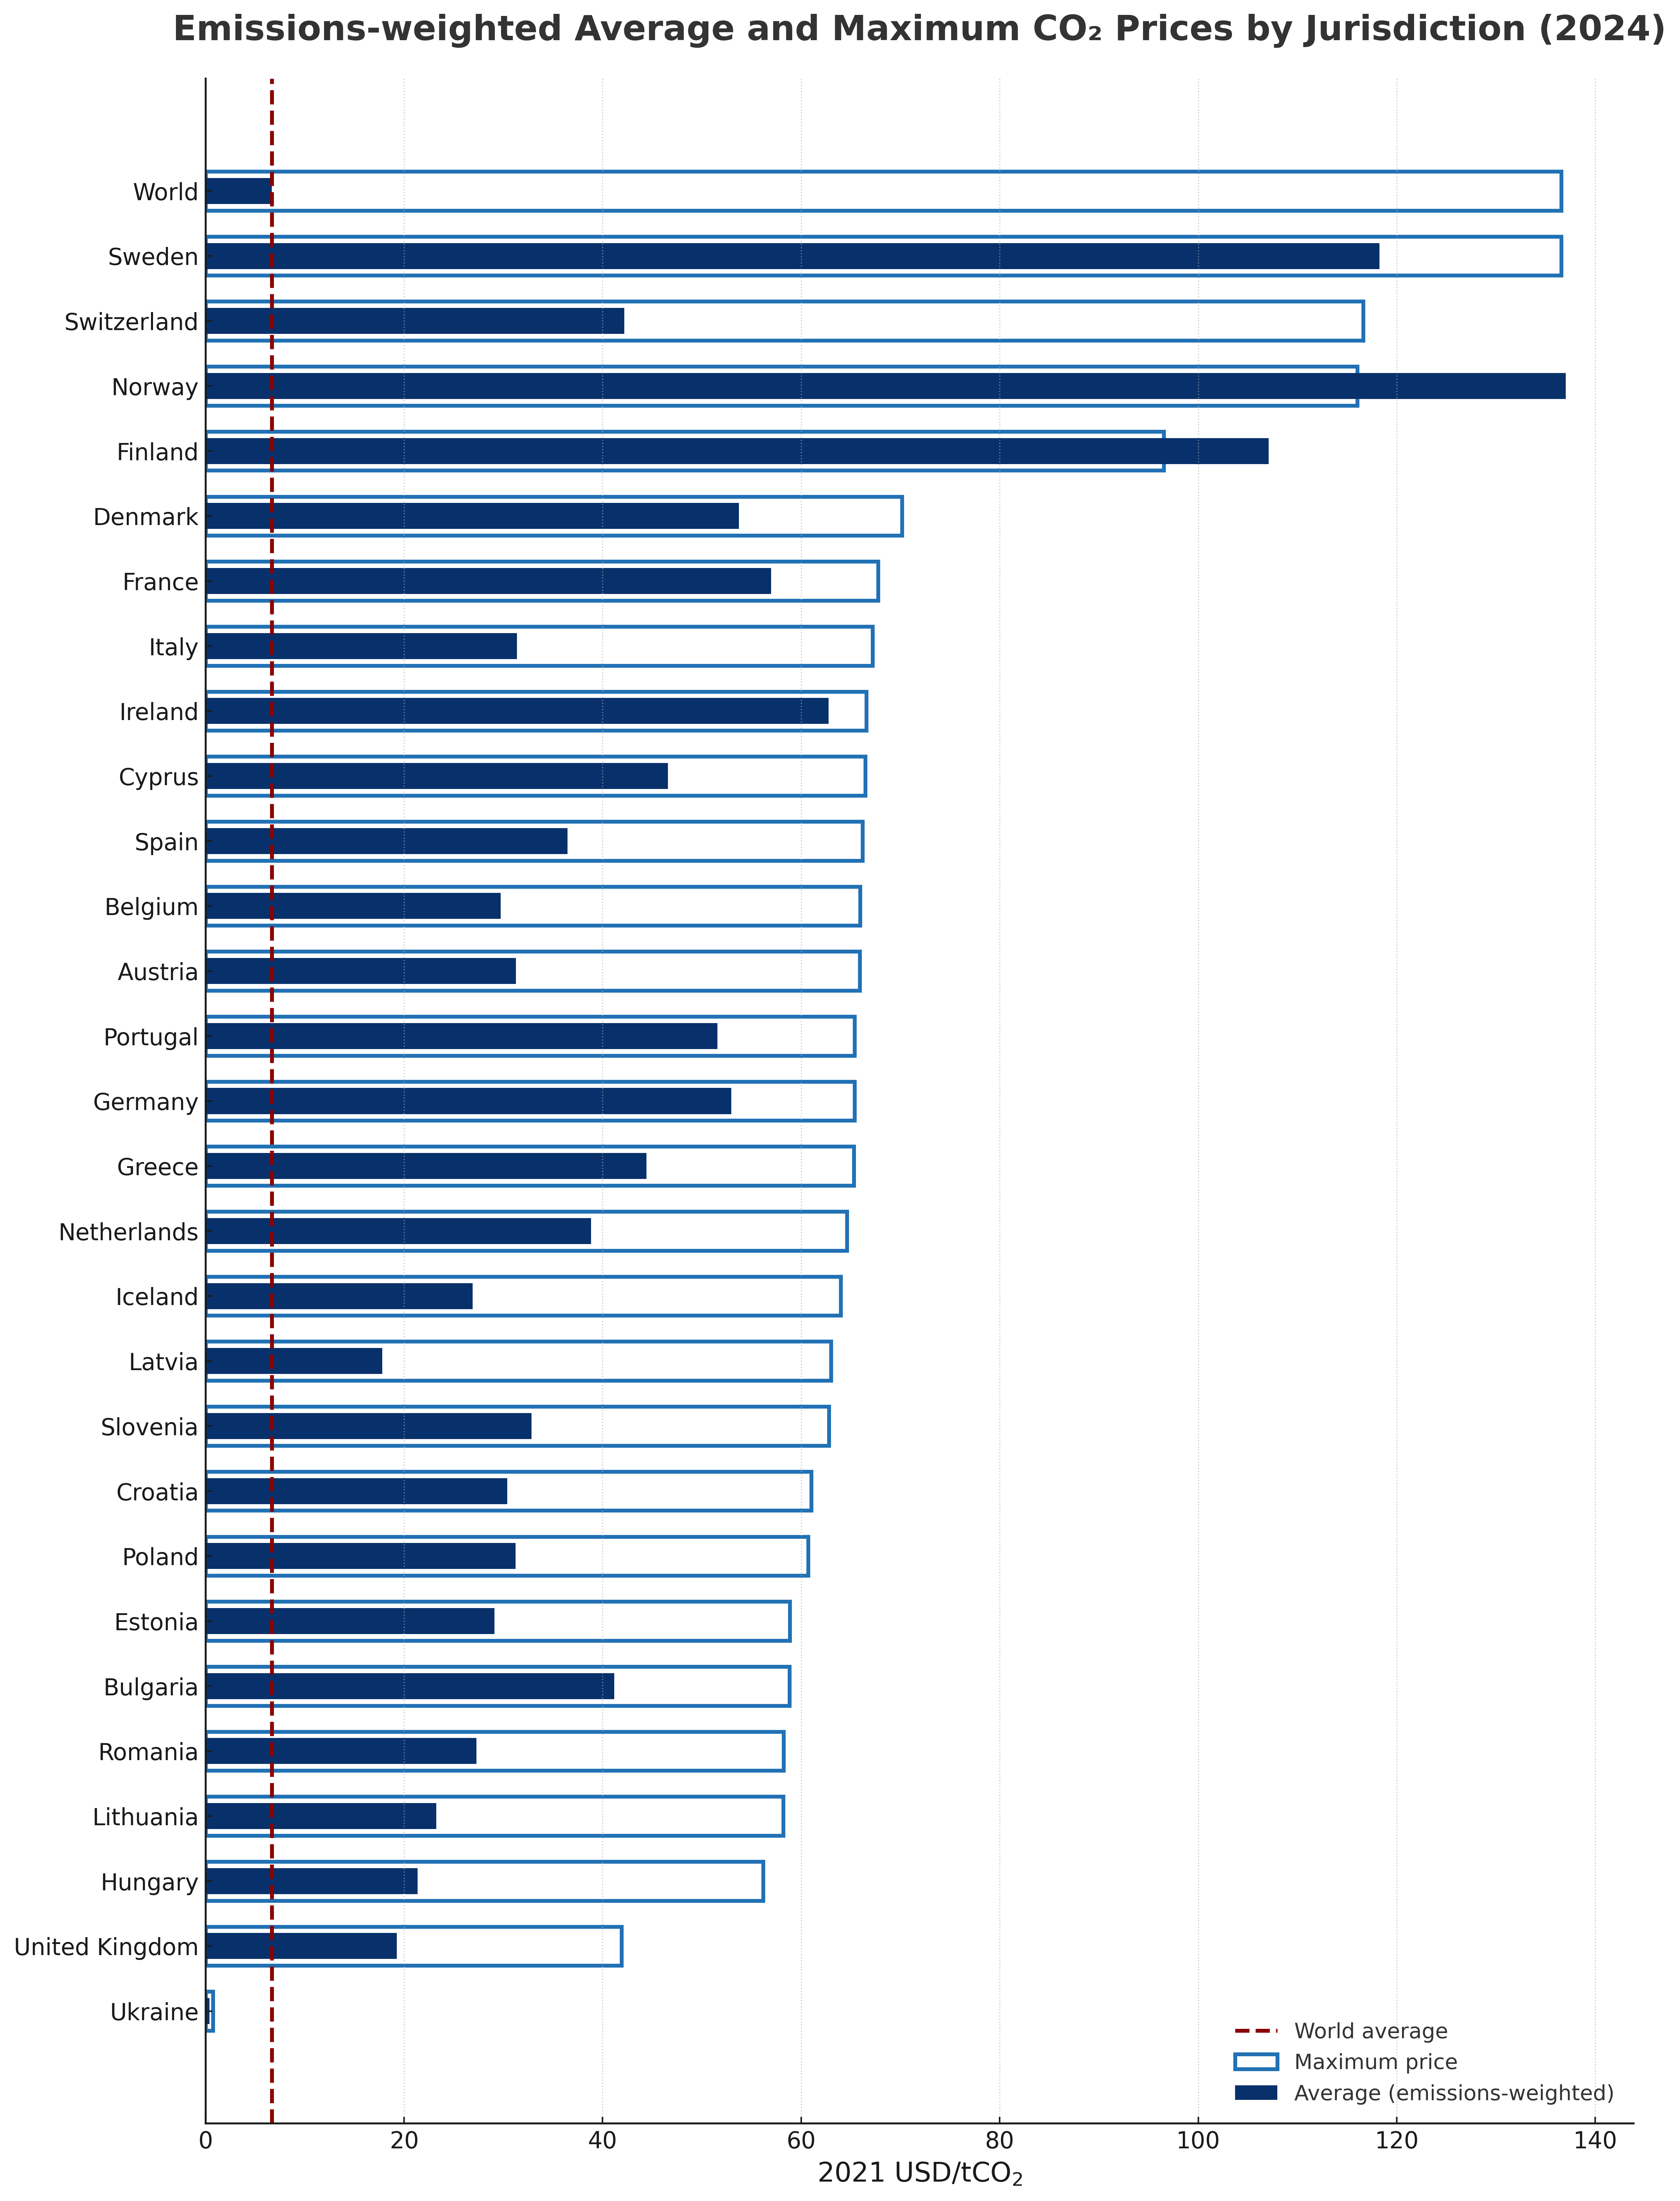
\includegraphics[keepaspectratio]{../../../_output/_figures/plots/max_price_ecp_2024_improved.png}}

}

\caption{\label{fig-avg-min}Maximum and average carbon prices, 2024}

\end{figure}%

\begin{figure}

\centering{

\pandocbounded{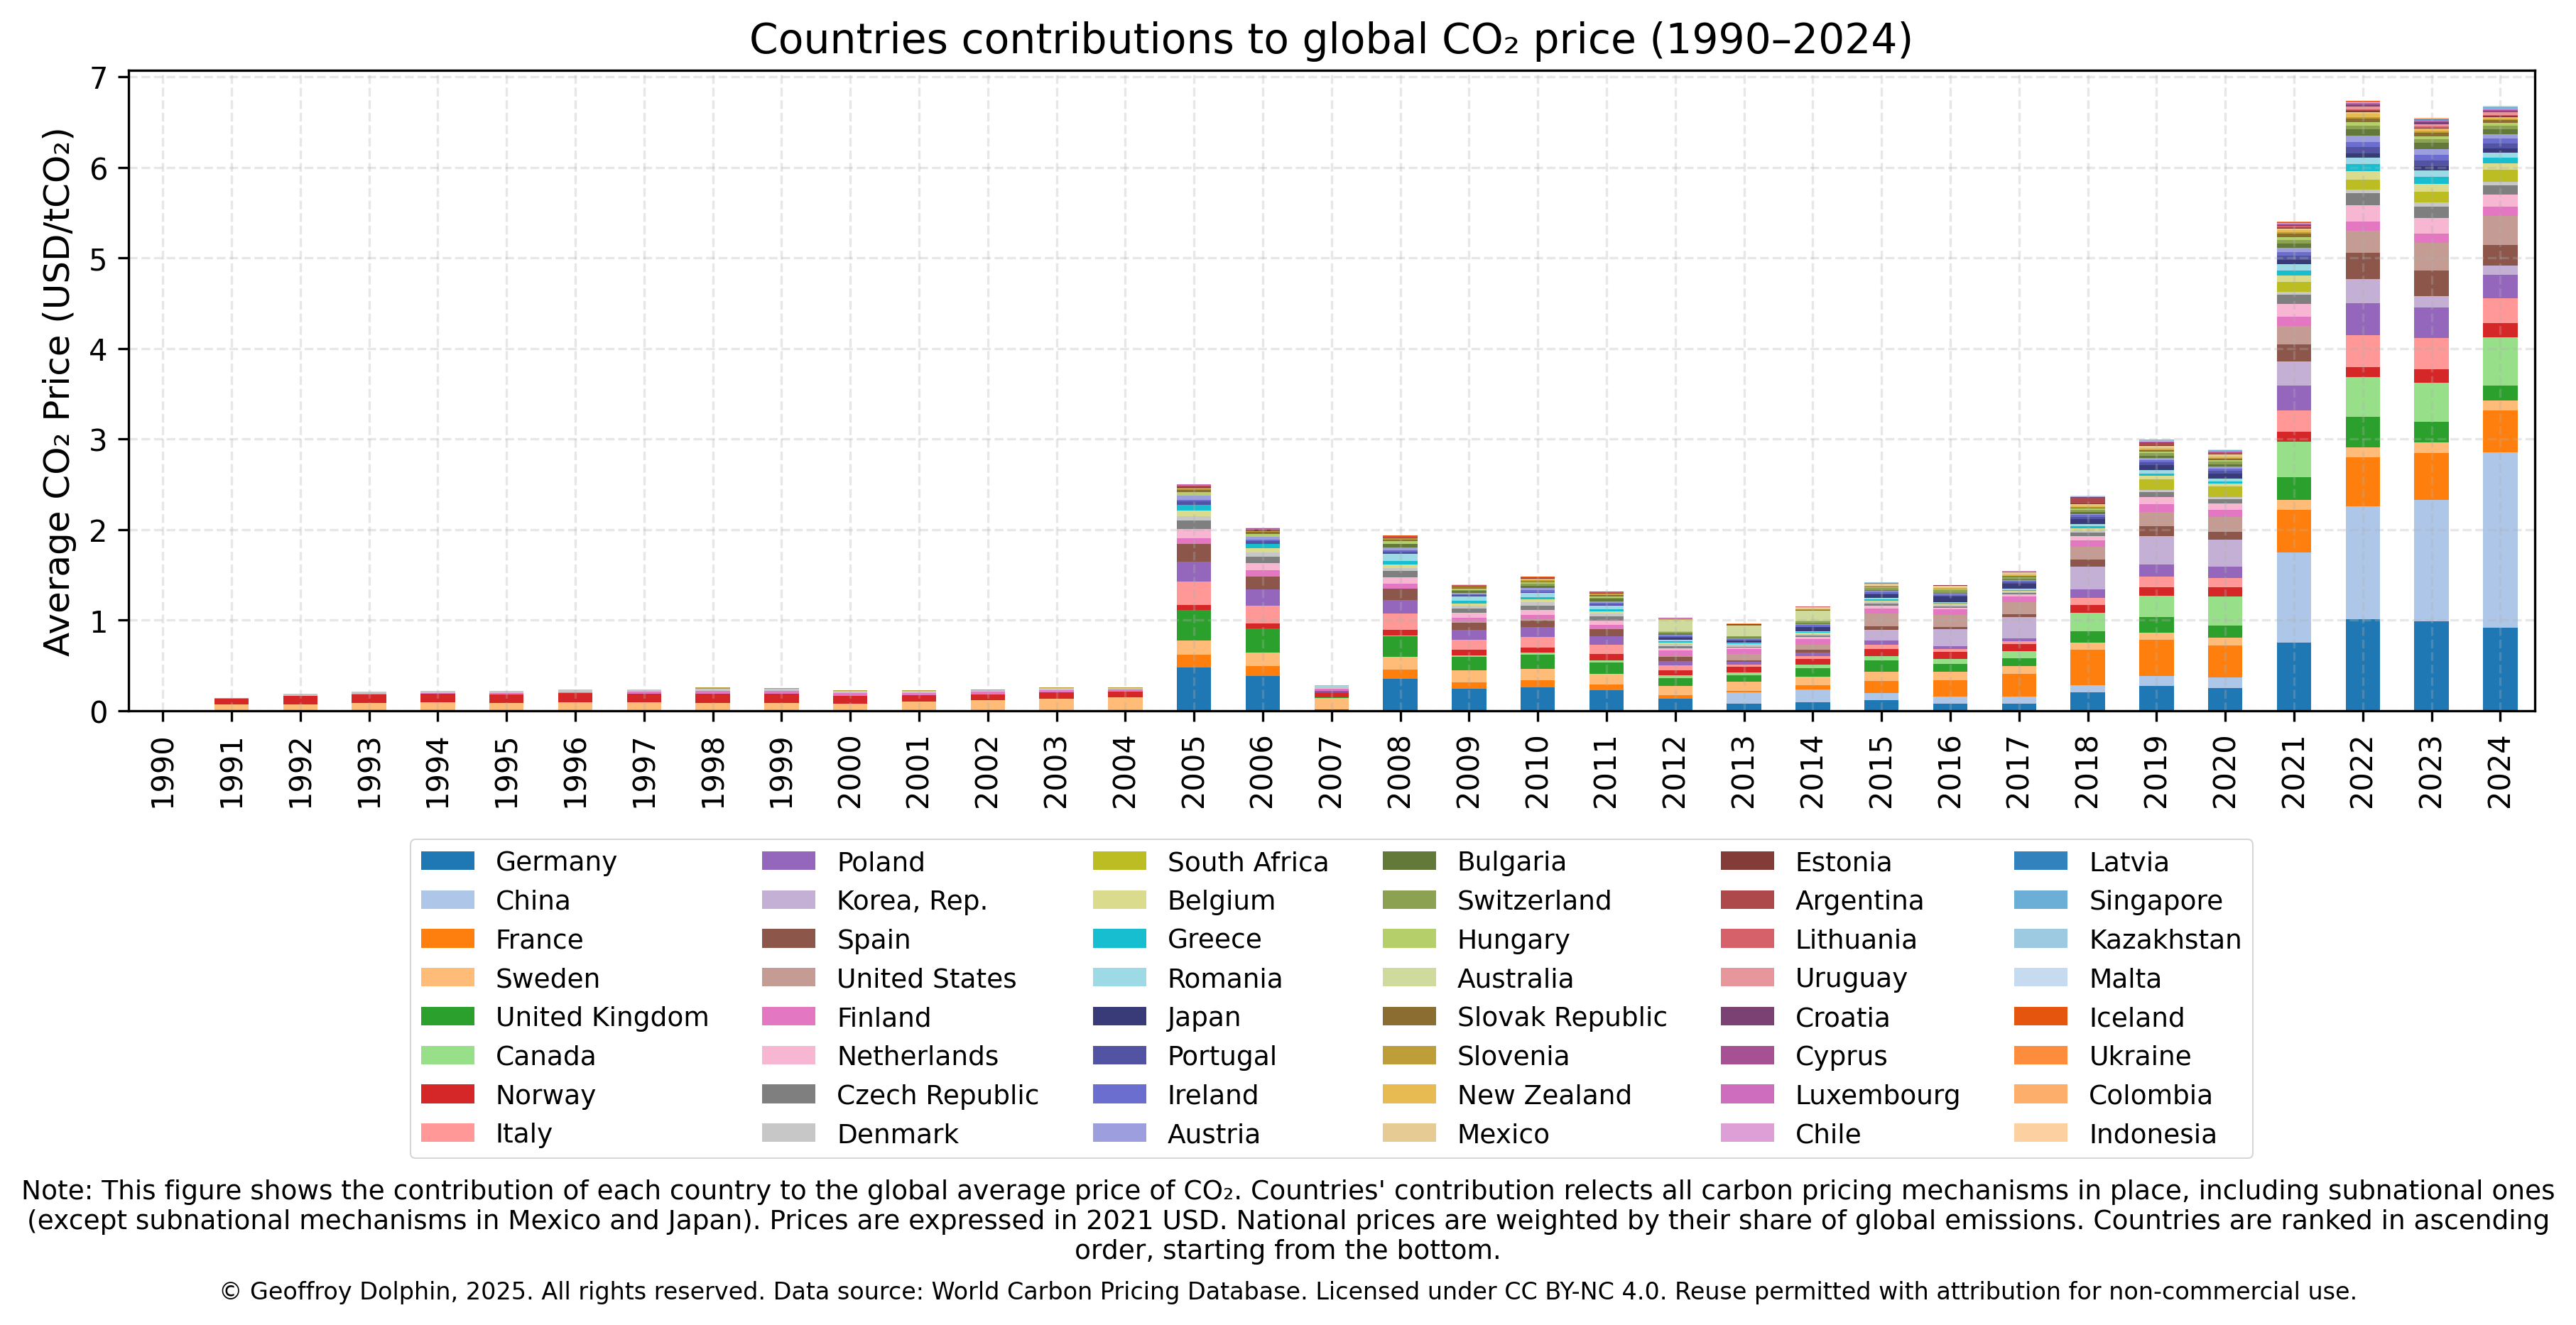
\includegraphics[keepaspectratio]{../../../_output/_figures/plots/national_stacked_world.png}}

}

\caption{\label{fig-nat-stacked-global}Contribution of countries to
global CO\(_2\) price, 1990-2024}

\end{figure}%

\begin{figure}

\centering{

\pandocbounded{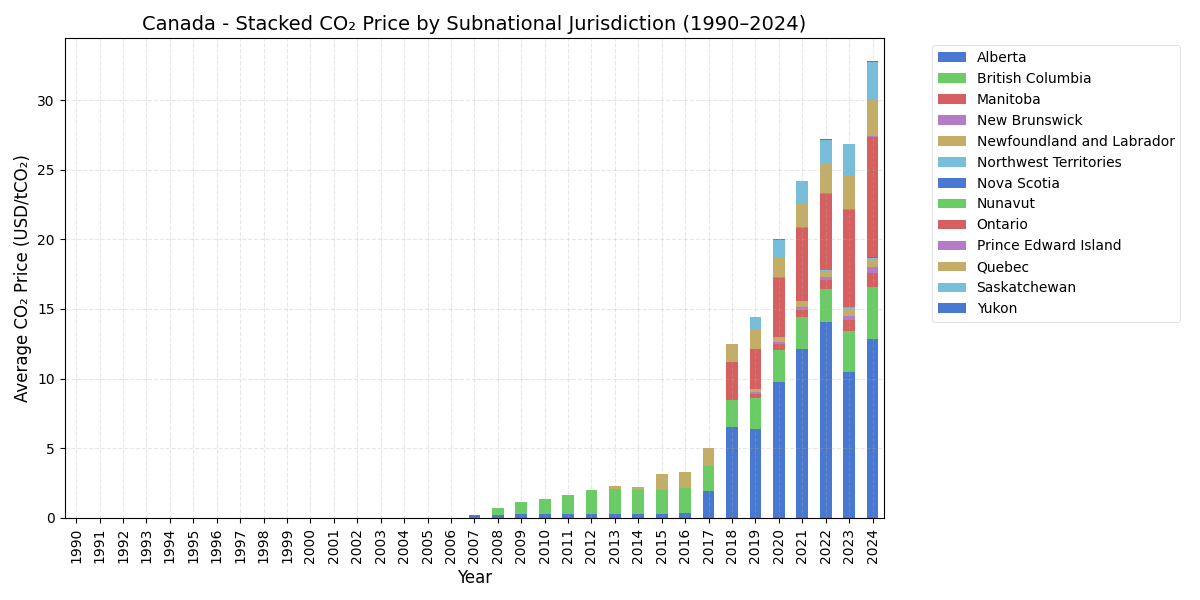
\includegraphics[keepaspectratio]{../../../_output/_figures/plots/subnat_stacked_Canada.png}}

}

\caption{\label{fig-subnat-stacked-canada}Contribution of subnational
jurisdictions to national average, Canada, 1990-2024}

\end{figure}%

\begin{figure}

\centering{

\pandocbounded{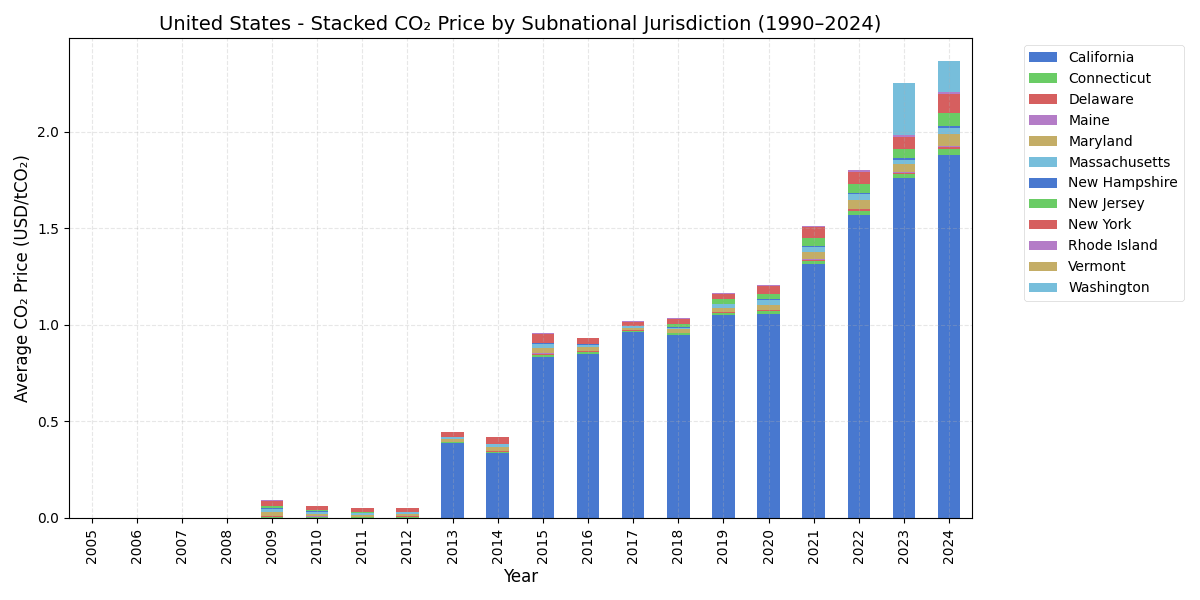
\includegraphics[keepaspectratio]{../../../_output/_figures/plots/subnat_stacked_United States.png}}

}

\caption{\label{fig-subnat-stacked-us}Contribution of subnational
jurisdictions to national average, United States, 1990-2024}

\end{figure}%

\begin{figure}

\centering{

\pandocbounded{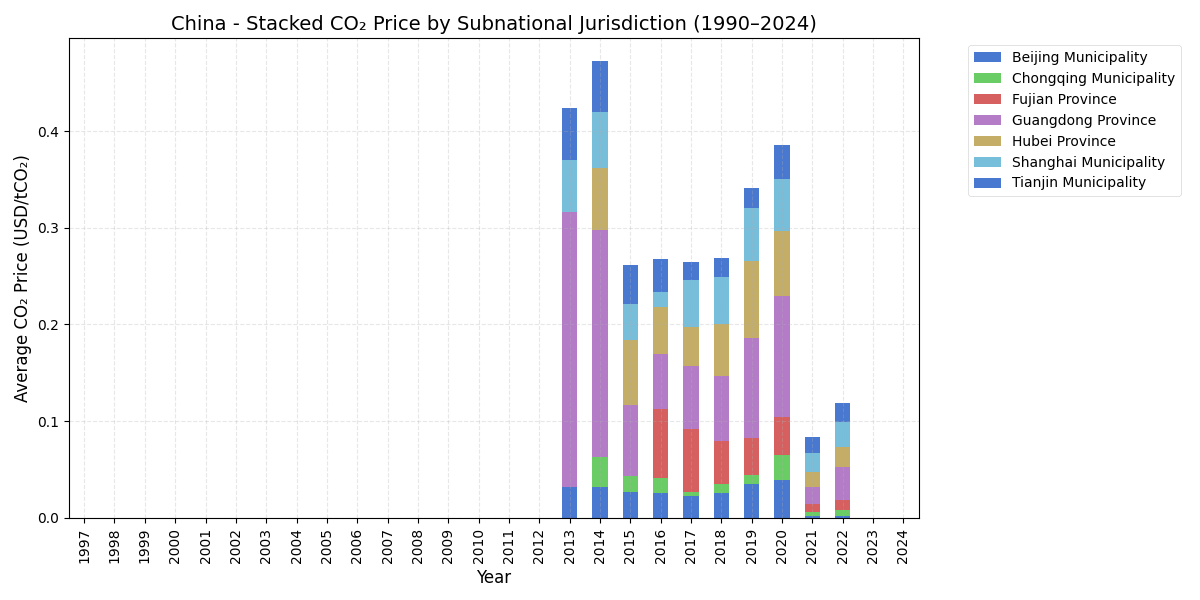
\includegraphics[keepaspectratio]{../../../_output/_figures/plots/subnat_stacked_China.png}}

}

\caption{\label{fig-subnat-stacked-china}Contribution of subnational
jurisdictions to national average, China, 1990-2024}

\end{figure}%

\newpage

\subsection{Carbon cost}\label{carbon-cost}

\begin{figure}

\centering{

\pandocbounded{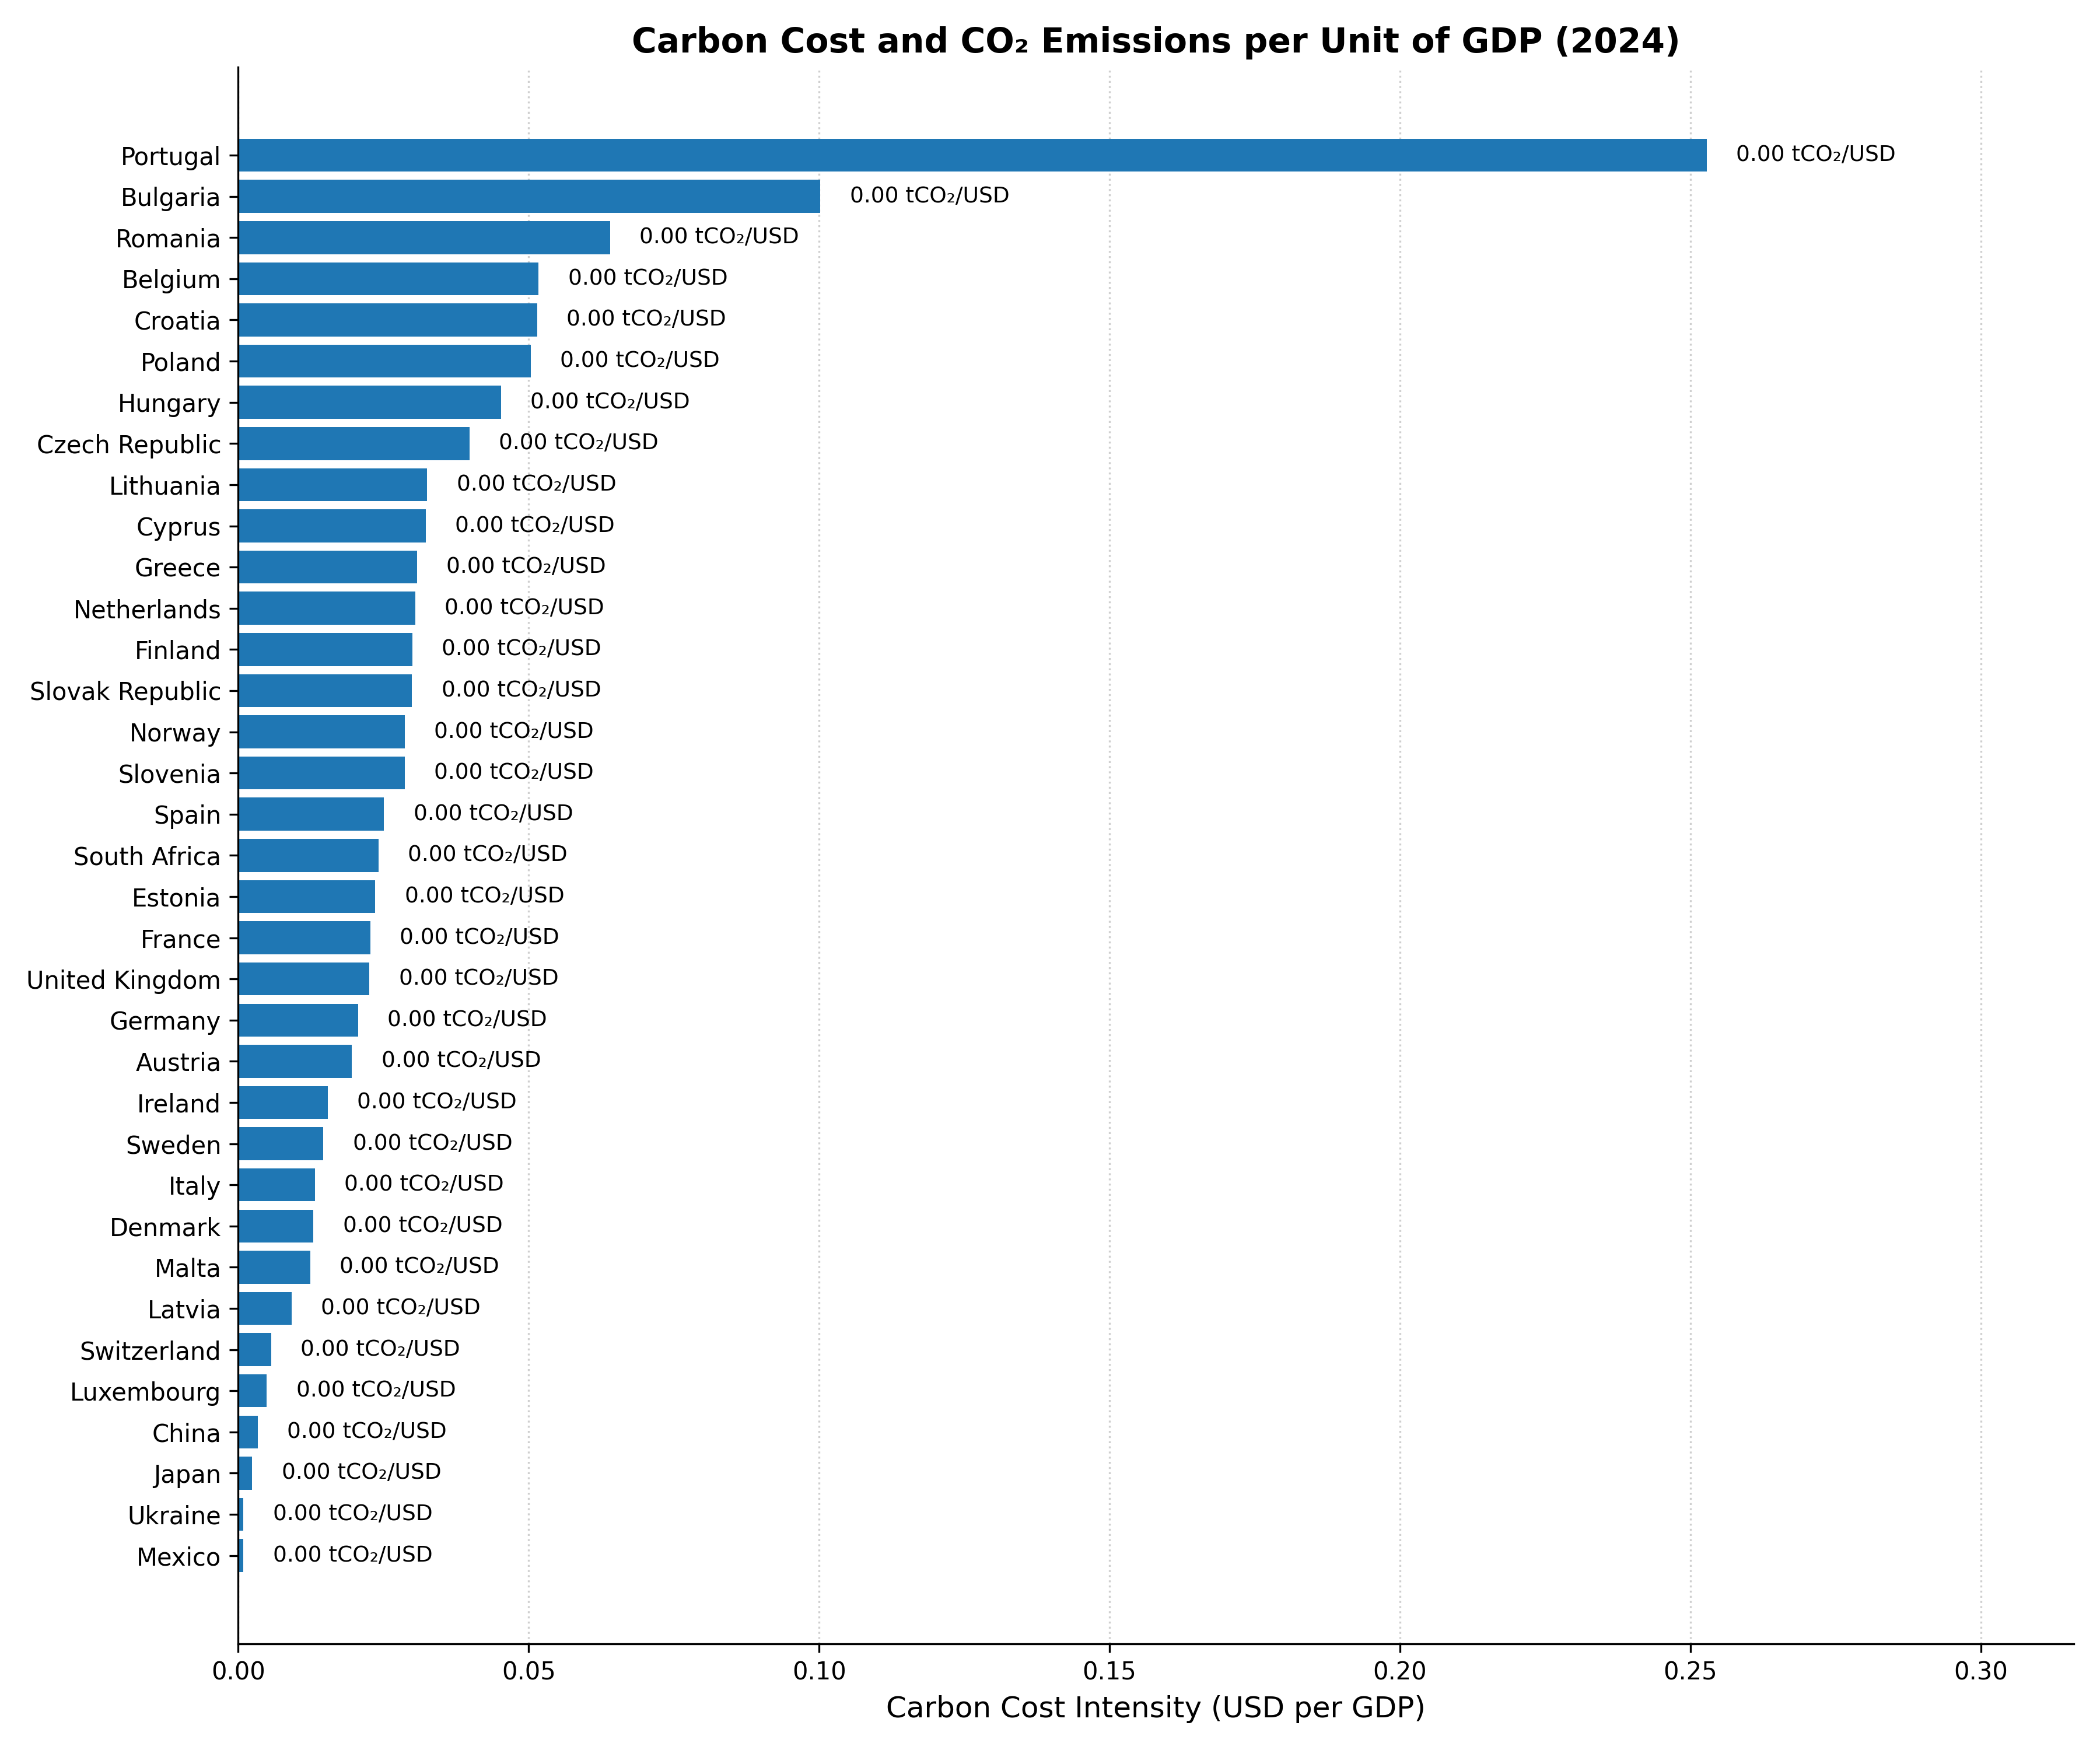
\includegraphics[keepaspectratio]{../../../_output/_figures/plots/carbon_cost.png}}

}

\caption{\label{fig-ccost}Carbon cost, 2021}

\end{figure}%

\newpage

\section{Country Fact Sheets}\label{country-fact-sheets}

\begin{verbatim}
Canada (2024):
    Average price = 32.80 USD/tCO2
    Maximum price = nan USD/tCO2
    Sectoral coverage (IPCC):

    Total coverage (CO2) = 0.45

China (2024):
    Average price = 5.92 USD/tCO2
    Maximum price = 13.22 USD/tCO2
    Sectoral coverage (IPCC):
            1A1A1, 1A1A2, 1A1A3
    Total coverage (CO2) = 0.45

France (2024):
    Average price = 56.97 USD/tCO2
    Maximum price = 67.74 USD/tCO2
    Sectoral coverage (IPCC):
            1A1A1, 1A1A2, 1A1A3, 1A1B, 1A1C, 1A2A, 1A2B, 1A2C, 1A2D
            1A2E, 1A2F, 1A2G, 1A2H, 1A2I, 1A2J, 1A2K, 1A2L, 1A2M
            1A3A1, 1A3A2, 1A3B, 1A3D2, 1A4A, 1A4B, 1C1A, 1C2B, 2A1
            2A2, 2A3, 2A4A, 2B1, 2B2, 2B3, 2B4, 2B5, 2B6
            2B7, 2B8F, 2C1, 2C2, 2C3, 2C4, 2C5, 2C6, 2H1
    Total coverage (CO2) = 0.87

Germany (2024):
    Average price = 52.98 USD/tCO2
    Maximum price = 65.38 USD/tCO2
    Sectoral coverage (IPCC):
            1A1A1, 1A1A2, 1A1A3, 1A1B, 1A1C, 1A2A, 1A2B, 1A2C, 1A2D
            1A2E, 1A2F, 1A2G, 1A2H, 1A2I, 1A2J, 1A2K, 1A2L, 1A2M
            1A3A1, 1A3A2, 1A3B, 1A3C, 1A3D2, 1A3E1, 1A4A, 1A4B, 1A4C1
            1A4C2, 1A4C3, 1A5A, 1A5B, 1C1A, 1C2B, 2A1, 2A2, 2A3
            2A4A, 2B1, 2B2, 2B3, 2B4, 2B5, 2B6, 2B7, 2B8F
            2C1, 2C2, 2C3, 2C4, 2C5, 2C6, 2H1
    Total coverage (CO2) = 0.90

Italy (2024):
    Average price = 31.36 USD/tCO2
    Maximum price = 67.18 USD/tCO2
    Sectoral coverage (IPCC):
            1A1A1, 1A1A2, 1A1A3, 1A1B, 1A1C, 1A2A, 1A2B, 1A2C, 1A2D
            1A2E, 1A2F, 1A2G, 1A2H, 1A2I, 1A2J, 1A2K, 1A2L, 1A2M
            1A3A1, 1A3A2, 1A3D2, 1C1A, 1C2B, 2A1, 2A2, 2A3, 2A4A
            2B1, 2B2, 2B3, 2B4, 2B5, 2B6, 2B7, 2B8F, 2C1
            2C2, 2C3, 2C4, 2C5, 2C6, 2H1
    Total coverage (CO2) = 0.42

Japan (2024):
    Average price = 1.78 USD/tCO2
    Maximum price = nan USD/tCO2
    Sectoral coverage (IPCC):
            1A1A1, 1A1A2, 1A1A3, 1A2A, 1A2B, 1A2C, 1A2D, 1A2E, 1A2F
            1A2G, 1A2H, 1A2I, 1A2J, 1A2K, 1A2L, 1A2M, 1A3B
    Total coverage (CO2) = 0.70

United Kingdom (2024):
    Average price = 19.25 USD/tCO2
    Maximum price = 41.90 USD/tCO2
    Sectoral coverage (IPCC):
            1A1A1, 1A1A2, 1A1A3, 1A1B, 1A1C, 1A2A, 1A2B, 1A2C, 1A2D
            1A2E, 1A2F, 1A2G, 1A2H, 1A2I, 1A2J, 1A2K, 1A2L, 1A2M
            1A3A2, 1C1A, 1C2B, 2A1, 2A2, 2A3, 2A4A, 2B1, 2B2
            2B3, 2B4, 2B5, 2B6, 2B7, 2B8F, 2C1, 2C2, 2C3
            2C4, 2C5, 2C6, 2H1
    Total coverage (CO2) = 0.46

United States (2024):
    Average price = 2.37 USD/tCO2
    Maximum price = nan USD/tCO2
    Sectoral coverage (IPCC):

    Total coverage (CO2) = 0.09
\end{verbatim}




\end{document}
